\documentclass[10pt, c, xcolor=x11names]{beamer}\usepackage[]{graphicx}\usepackage[]{color}
%% maxwidth is the original width if it is less than linewidth
%% otherwise use linewidth (to make sure the graphics do not exceed the margin)
\makeatletter
\def\maxwidth{ %
  \ifdim\Gin@nat@width>\linewidth
    \linewidth
  \else
    \Gin@nat@width
  \fi
}
\makeatother

\definecolor{fgcolor}{rgb}{0.345, 0.345, 0.345}
\newcommand{\hlnum}[1]{\textcolor[rgb]{0.686,0.059,0.569}{#1}}%
\newcommand{\hlstr}[1]{\textcolor[rgb]{0.192,0.494,0.8}{#1}}%
\newcommand{\hlcom}[1]{\textcolor[rgb]{0.678,0.584,0.686}{\textit{#1}}}%
\newcommand{\hlopt}[1]{\textcolor[rgb]{0,0,0}{#1}}%
\newcommand{\hlstd}[1]{\textcolor[rgb]{0.345,0.345,0.345}{#1}}%
\newcommand{\hlkwa}[1]{\textcolor[rgb]{0.161,0.373,0.58}{\textbf{#1}}}%
\newcommand{\hlkwb}[1]{\textcolor[rgb]{0.69,0.353,0.396}{#1}}%
\newcommand{\hlkwc}[1]{\textcolor[rgb]{0.333,0.667,0.333}{#1}}%
\newcommand{\hlkwd}[1]{\textcolor[rgb]{0.737,0.353,0.396}{\textbf{#1}}}%
\let\hlipl\hlkwb

\usepackage{framed}
\makeatletter
\newenvironment{kframe}{%
 \def\at@end@of@kframe{}%
 \ifinner\ifhmode%
  \def\at@end@of@kframe{\end{minipage}}%
  \begin{minipage}{\columnwidth}%
 \fi\fi%
 \def\FrameCommand##1{\hskip\@totalleftmargin \hskip-\fboxsep
 \colorbox{shadecolor}{##1}\hskip-\fboxsep
     % There is no \\@totalrightmargin, so:
     \hskip-\linewidth \hskip-\@totalleftmargin \hskip\columnwidth}%
 \MakeFramed {\advance\hsize-\width
   \@totalleftmargin\z@ \linewidth\hsize
   \@setminipage}}%
 {\par\unskip\endMakeFramed%
 \at@end@of@kframe}
\makeatother

\definecolor{shadecolor}{rgb}{.97, .97, .97}
\definecolor{messagecolor}{rgb}{0, 0, 0}
\definecolor{warningcolor}{rgb}{1, 0, 1}
\definecolor{errorcolor}{rgb}{1, 0, 0}
\newenvironment{knitrout}{}{} % an empty environment to be redefined in TeX

\usepackage{alltt}

\def\currentChapter{Biological Network Inference with Sparse Graphical Models}


% THEME BEAMER
\usepackage{../themeJC2BIM}

\graphicspath{{figures/},{../common_figs/}}
\usepackage{tikz}
\usetikzlibrary{calc,shapes,backgrounds,arrows,automata,shadows,positioning}
\tikzstyle{every state}=[fill=red,draw=none,scale=0.7,font=\small,text=white]
\tikzstyle{every edge}=[-,shorten >=1pt,auto,thin,draw]
\tikzstyle{alertstate}=[fill=bleu]
\definecolor{genecolor}{RGB}{94,135,173}

\def\currentDate{Fréjus, 4--8 June 2018}
\def\currentInstitute{Julien Chiquet}
\def\currentCourse{(JC)2BIM 2018 Research School}

\title{\currentCourse}

\subtitle{\huge\currentChapter\normalsize}

\institute{\currentInstitute}

\date{\currentDate}



\AtBeginSection{
  \begin{frame}<beamer>
    \frametitle{Outline}
    \framesubtitle{\insertpart}
    \tableofcontents[currentsection,currentsubsection, subsectionstyle=show/shaded/hide]  
  \end{frame}
}

\AtBeginSubsection{
  \begin{frame}<beamer>
    \frametitle{Outline}
    \framesubtitle{\insertpart}
    \tableofcontents[currentsection,currentsubsection, subsectionstyle=show/shaded/hide]  
  \end{frame}
}

\AtBeginSubsubsection{
  \begin{frame}<beamer>
    \frametitle{Outline}
    \framesubtitle{\insertpart}
    \tableofcontents[currentsection,currentsubsection, subsectionstyle=show/shaded/hide]  
  \end{frame}
}

\newcommand{\dotitlepage}{%
  \begin{frame}
    \titlepage
    \vfill
    \begin{center}
        \scriptsize\url{https://github.com/jchiquet/JC2BIM18}
    \end{center}
    \vfill
    
\includegraphics[width=1.5cm]{logo_cnrs}\hfill
    
\includegraphics[width=2.5cm]{logo_inra}
  \end{frame}
  %
}

\newcommand{\dotoc}{%
  \begin{frame}
    \frametitle{Outline}
    \tableofcontents[currentsection,
    sectionstyle=show/show,
    subsectionstyle=hide]
  \end{frame}
  %
}

\usepackage{hhline}



\pgfdeclareimage[width=.3\textwidth]{affymetrix}{../common_figs/tech_affy}
\pgfdeclareimage[width=.18\textwidth]{microarray}{../common_figs/data_affy}
\pgfdeclareimage[width=.18\textwidth]{sequencer}{../common_figs/tech_ngs}
\pgfdeclareimage[width=.25\textwidth]{ngs}{../common_figs/data_ngs}
\pgfdeclareimage[width=.5cm]{computer}{../common_figs/computer}
\IfFileExists{upquote.sty}{\usepackage{upquote}}{}
\begin{document}

\part<presentation*>{Introduction}

\dotitlepage

\dotoc

\begin{frame}
  \frametitle{Omic: parallel measurement of \alert{many} biological features}

  Focus e.g. on \textit{transcription},    looking toward \textcolor{genecolor}{\textit{gene regulatory networks}}

  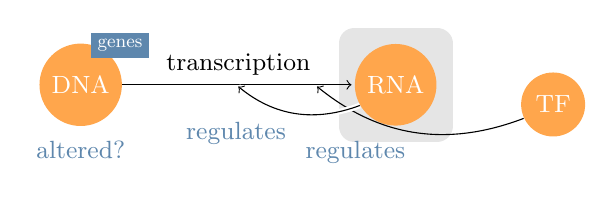
\begin{tikzpicture}
    \begin{small}
      \tikzstyle{every state}=[fill=orange!70!white,draw=none,text=white]
      \node[state] (dna) at (0,0) {DNA};
      \node[state] (rna) at (4,0) {RNA};
      \node[state] (tf) at (6,-0.25) {TF};
      \node[draw=none,text=white,fill=genecolor, scale=0.75] (gene) at (0.5,0.5) {genes};
      \node[draw=none,text=genecolor,fill=white] (alter) at ($(dna.south) -(0,3mm)$) {altered?};

      \path
      (dna) edge [->] node[above] {\alert{transcription}} (rna)
      (tf) edge [bend left, ->] node[midway] {\textcolor{genecolor}{regulates}} ($(rna.west) -(5mm,0)$)
      (rna) edge [-,line width=2pt,draw=white,bend left] ($(rna.west) -(15mm,0)$)
      (rna) edge [bend left, ->] node {\textcolor{genecolor}{regulates}} ($(rna.west) -(15mm,0)$);
    \end{small}

    \begin{pgfonlayer}{background}
      \filldraw [line width=4mm,join=round,black!10]
      (rna.north -| rna.west) rectangle (rna.south -| rna.east);
    \end{pgfonlayer}

  \end{tikzpicture}

  \only<1>{
    \begin{tikzpicture}
      \node at (0,-.25) {\pgfuseimage{affymetrix}};
      \node[fill=mred, text=white,single arrow]
      (sig) at (3.5,-.25) {\sf \scriptsize signal processing};
      \node[opacity=.75] (array1) at (7.25,0.25) {\pgfuseimage{microarray}};
      \node[opacity=.9] (array2) at (7.5,0) {\pgfuseimage{microarray}};
      \node[opacity=.95] (array3) at (7.75,-0.25) {\pgfuseimage{microarray}};
      \node at (8,-0.5) (array4) {\pgfuseimage{microarray}};

      \begin{pgfonlayer}{background}
        \filldraw [line width=4mm,join=round,black!10]
        (array1.north -| array1.west) rectangle (array4.south -| array4.east);
      \end{pgfonlayer}

      \node at (7,-3) {%
        $\mathbf{X} = \begin{pmatrix}
          x_1^1 & x_1^2 & x_1^3 & \dots & x_1^p \\
          \vdots \\
          x_n^1 & x_n^2 & x_1^2 & \dots & x_n^p \\
        \end{pmatrix}$};

      \node (output) at (0,-3) {
        \begin{tabular}{@{}l@{}}
          \small Matrix of features $n\ll p$\\ \hline
          \scriptsize Expression levels of $p$ \\
          \scriptsize probes are simultaneously \\
          \scriptsize monitored for $n$ individuals
        \end{tabular}
      };

      \begin{pgfonlayer}{background}
        \filldraw [line width=4mm,join=round,black!10]
        (output.north -| output.west) rectangle (output.south -| output.east);
      \end{pgfonlayer}

      \node[fill=mred, text=white,single arrow, shape border rotate =180]
      (inference) at (3.35,-3) {\sf \scriptsize pretreatment};
    \end{tikzpicture}
  }

  \only<2>{
    \begin{tikzpicture}
      \node at (0,-.25) {\pgfuseimage{sequencer}};

      \node[fill=mred, text=white,single arrow]
      (sig) at (3.5,-.25) {\sf \scriptsize assembling};

      \node[opacity=.75] (array1) at (7.25,0.25) {\pgfuseimage{ngs}};
      \node[opacity=.9] (array2) at (7.5,0) {\pgfuseimage{ngs}};

      \begin{pgfonlayer}{background}
        \filldraw [line width=4mm,join=round,black!10]
        (array1.north -| array1.west) rectangle (array2.south -| array2.east);
      \end{pgfonlayer}

      \node at (7,-2.75) {%
        $\mathbf{X} = \begin{pmatrix}
          k_1^1 & k_1^2 & k_1^3 & \dots & k_1^p \\
          \vdots \\
         k_n^1 & k_n^2 & k_1^2 & \dots & k_n^p \\
        \end{pmatrix}$};

      \node (output) at (0,-2.75) {
        \begin{tabular}{@{}l@{}}
          \small Matrix of features $n\lll p$\\ \hline
          \scriptsize Expression counts are extracted \\
          \scriptsize from small repeated sequences \\
          \scriptsize and monitored for $n$ individuals
        \end{tabular}
      };

      \begin{pgfonlayer}{background}
        \filldraw [line width=4mm,join=round,black!10]
        (output.north -| output.west) rectangle (output.south -| output.east);
      \end{pgfonlayer}

      \node[fill=mred, text=white,single arrow, shape border rotate =180]
      (inference) at (3.35,-2.75) {\sf \scriptsize pretreatment};
    \end{tikzpicture}
    }
\end{frame}

\begin{frame}
  \frametitle{Network inference: a challenging problem}

  \begin{columns}[c]
    \begin{column}{.55\textwidth}
      \begin{tikzpicture}[scale=0.75]
        \node[scale=0.75,opacity=0.75] at (-3,3) {\pgfuseimage{sequencer}};
        \node[scale=0.75] at (-3.5,1) {\pgfuseimage{affymetrix}};
        \node[scale=0.75,fill=red, text=white,single arrow]
        (inference) at (-1.7,1.7) {\sf \scriptsize Inference};

        \node at (-3,-0.5) {\begin{tabular}{@{}c@{}}
            \tiny $\approx$ 10s/1,000s assays \\
            \tiny $\approx $ 1,000s/1,000,000s features \\
          \end{tabular}
        };

        %% UN GRAPH
        \tikzstyle{every edge}=[-,>=stealth',shorten >=1pt,auto,thin,draw,color=genecolor]
        \tikzstyle{every node}=[fill=genecolor]
        \tikzstyle{every state}=[draw=none,text=white,scale=0.5, transform shape]

        % premier cluster
        \node[state] (A1) at (0,1.75) {g1};
        \node[state] (A2) at (1,0.75) {g2};
        \node[state] (A3) at (0,-.25) {g3};
        \node[state] (A4) at (-1,0.75) {g4};
        \node[state] (A5) at (0,0.75) {g5};

        \foreach   \name/\angle/\text   in  {B1/234/g6,   B2/162/g7,
          B3/90/g8, B4/18/g9, B5/-54/g10} {
          \node[state,xshift=4cm,yshift=4cm]     (\name)    at
          (\angle:1cm) {\text}; }

        \node[state] (B6) at (2,2) {g11};
        \node[state] (C1) at (3,0.5) {g12};
        \node[state] (C2) at (2.2,0) {g13};

        \path
        (A5) edge [bend left] (A1)
        (A5) edge [bend left] (A2)
        (A5) edge [bend left] (A3)
        (A5) edge [bend left] (A4)
        (B6) edge [bend right] (B1)
        (B6) edge [bend right] (B2)
        (B6) edge [bend right] (B3)
        (B6) edge [bend right] (B4)
        (B6) edge [bend right] (B5)
        (C2) edge [bend left] (C1)
        (A5) edge [bend left] (B6)
        (B6) edge [bend right] (C2);
      \end{tikzpicture}
    \end{column}
    \begin{column}{.45\textwidth}
      \begin{footnotesize}
        \begin{enumerate}
        \item Nodes are fixed
            \noindent\begin{itemize}
            \item \scriptsize \alert{restricted}   to  a   set  of   interest
            \end{itemize}
        \item Edges (interactions) are inferred
          \begin{scriptsize}
            \begin{itemize}
            \item \scriptsize based upon \alert{statistical} concepts
            \end{itemize}
          \end{scriptsize}
        \end{enumerate}
      \end{footnotesize}
    \end{column}
  \end{columns}

  \begin{block}{Statistical question}
    \vspace{-.25cm}
    \begin{enumerate}
    \item Variable selection (which edges?)
    \end{enumerate}
  \end{block}

  \begin{block}{Main statistical challenges}
    \vspace{-.25cm}
    \begin{enumerate}
    \item (Ultra) High dimensionality ($n<p$, $n\lll p$)
    \item Heterogeneity/structure of the data
    \end{enumerate}
  \end{block}

\end{frame}



\begin{frame}
  \frametitle{Outline}

  \begin{enumerate}
  \item[Part 1] \alert{Framework}\\
    \textit{Gaussian graphical models and sparse regularization techniques}\bigskip

  \item[Part 2] \alert{Extensions}\\
    \textit{Extensions of these methods for omic data analyses}\bigskip

  \end{enumerate}
\end{frame}

\AtBeginSection[]{
  \begin{frame}<handout:0>
    \frametitle{Outline}
    \tableofcontents[currentsection]
  \end{frame}
}

\part<presentation>{sparse Gaussian Graphical Models}
\begin{frame}
  \partpage
  \tableofcontents[hideallsubsections]
\end{frame}

\begin{frame}
  \frametitle{Outline}
  \tableofcontents
\end{frame}
 
\section{Network Inference}

\pgfdeclareimage[height=0.8\textheight]{sparsity1}{figures/sparsity_1}
\pgfdeclareimage[height=0.8\textheight]{sparsity2}{figures/sparsity_2}
\pgfdeclareimage[height=0.375\textheight]{sparsity4}{figures/sparsity_4}

\begin{frame}
  \frametitle{References}

    \begin{thebibliography}{99}
      \setbeamertemplate{bibliography item}[book]

    \bibitem[JC]{JC} Habilitation, J. Chiquet, Chapter 2 \href{https://tel.archives-ouvertes.fr/tel-01288976/}{https://tel.archives-ouvertes.fr/tel-01288976/}
    \bibitem[EI]{EI} The Element of Statistical Learning \textcolor{black}{Hastie, Tibshirani, Friedman}, chapter 17.
    \end{thebibliography}

\end{frame}

\begin{frame}
  \frametitle{Some families of methods for network reconstruction}

  \begin{block}{Test-based methods}
    \vspace{-.15cm}
    \begin{itemize}
    \item Tests the nullity of each entries 
    \item Combinatorial problem when $p>30$ \dots
    \end{itemize}    
  \end{block}
  
  \vfill

  \begin{block}{Bayesian methods}
    \vspace{-.15cm}
    \begin{itemize}
    \item Compute the posterior probability of each edge
    \item Usually more computationally demanding
    \item For special graphs, computation gets easier
    \end{itemize}
  \end{block}

  \begin{block}{\alert{Sparsity-inducing regularization methods}}
    \vspace{-.15cm}
    \begin{itemize}
    \item induce sparsity with the $\ell_1$-norm penalization
    \item Use results from convex optimization
    \item Versatile and computationally efficient
    \end{itemize}
  \end{block}

\end{frame}

\subsection{Inducing sparsity for edge selection}

\begin{frame}
  \frametitle{Inference: maximum likelihood estimator}
  \framesubtitle{The natural approach for parametric statistics}

  Let   $X\sim f_{X}(x;\boldsymbol\Omega)$,  where   $\boldsymbol\Omega$  are  the
  model parameters.

  \vfill

  \begin{block}{Maximum likelihood estimator}
    \begin{equation*}
      \hat{\boldsymbol\Omega}      =      \argmax_{\boldsymbol\Omega}
      \ell(\boldsymbol\Omega; \mathbf{X})
    \end{equation*}
    where  $\ell$ is  the log  likelihood, a  function  of the
    parameters:
    \begin{equation*}
      \ell(\boldsymbol\Omega;      \mathbf{X})      =     \log
      \prod_{i=1}^n f_{X}(\mathbf{x}_i;\boldsymbol\Omega),
    \end{equation*}
    where $\mathbf{x}_i$ is the $i$th row of $\mathbf{X}$.
  \end{block}

  \vfill
  
  \begin{itemize}
    \item This a convex optimization problem,
    \item We just need to detect non zero coefficients in $\boldsymbol\Omega$
  \end{itemize}

\end{frame}

\begin{frame}
  \frametitle{The multivariate Gaussian log-likelihood }

  Let  $\mathbf{S}  =  n^{-1}\mathbf{X}^\intercal \mathbf{X}$  be  the
  empirical variance-covariance  matrix: $\mathbf{S}$ is  a sufficient
  statistic of $ \boldsymbol\Omega$.

  \vfill

  \begin{block}{The log-likelihood}
    \begin{equation*}
      \ell(\boldsymbol\Omega; \mathbf{S}) =
      \frac{n}{2}     \log    \det     (\boldsymbol\Omega)  - \frac{n}{2}
      \mathrm{Trace}(\mathbf{S} \boldsymbol\Omega) + \frac{n}{2}\log(2\pi).
    \end{equation*}
  \end{block}

  \vfill

  \begin{itemize}
  \item[$\rightsquigarrow$]    The     MLE    $=\mathbf{S}^{-1}$    of
    $\boldsymbol\Omega$ is not defined for $n< p$ and never sparse.
  \item[$\rightsquigarrow$] The need for regularization is huge.
  \end{itemize}
\end{frame}

\begin{frame}
  \frametitle{A Geometric View of Shrinkage}
  \framesubtitle{Constrained Optimization}

  \begin{overlayarea}{\textwidth}{\textheight}
    \begin{columns}
      \begin{column}{0.475\textwidth}
        \begin{tikzpicture}
          \only<1>{%
            \node (Surf) at (0,0) {\pgfuseimage{sparsity1}}
            node     at    (Surf.west)    [rotate=90,yshift=5mm]
            {$L(\Omega_1,\Omega_2;\mathbf{X})$}
            node at (Surf.south west) [xshift=5mm,yshift=5mm]{$\Omega_2$}
            node at (Surf.south east) [xshift=-7.5mm,yshift=2.5mm]{$\Omega_1$};
          }
          \only<2>{%
            \node (Surf2) at (0,0) {\pgfuseimage{sparsity2}}
            node    at    (Surf2.west)    [rotate=90,yshift=5mm]
            {$L(\Omega_1,\Omega_2;\mathbf{X})$}
            node at (Surf2.south west) [xshift=5mm,yshift=5mm]{$\Omega_2$}
            node at (Surf2.south east) [xshift=-7.5mm,yshift=2.5mm]{$\Omega_1$};
          }
          \only<3->{%
            \node (titi) at (0,0) {\phantom{titi}};
            \node (Surf3) at (0,-4.5) {\pgfuseimage{sparsity4}}
            node at (Surf3.west) [rotate=90,yshift=2.5mm] {$\Omega_2$}
            node at (Surf3.south) [yshift=-2.5mm] {$\Omega_1$};
          }
        \end{tikzpicture}
      \end{column}
      \begin{column}{0.55\textwidth}
        \only<1>{%
          We basically want to solve a problem of the form
          \begin{equation*}
            \maximize_{\Omega_1,\Omega_2} \ell(\Omega_1,\Omega_2;\mathbf{X})
          \end{equation*}
          where $\ell$ is typically a concave likelihood function.
        }
        \only<2->{%
          \begin{equation*}
            \left\{\begin{array}{ll}
                \displaystyle    \maximize_{\Omega_1,\Omega_2}   &
                \ell(\Omega_1,\Omega_2;\mathbf{X})\\
                \mathrm{s.t.} & \Omega(\Omega_1,\Omega_2) \leq c
              \end{array}\right.,
          \end{equation*}
          where  $\Omega$  defines  a  domain  that  \textit{constrains}
          $\boldsymbol\beta$.

          \begin{center}
            How shall we define $\Omega$ ?
          \end{center}
        }
      \end{column}
    \end{columns}
  \end{overlayarea}
\end{frame}


\pgfdeclareimage[height=0.375\textheight]{sparsity6}{figures/sparsity_6}
\pgfdeclareimage[height=0.375\textheight]{sparsity8bis}{figures/sparsity_8bis}
\pgfdeclareimage[height=0.375\textheight]{sparsity9}{figures/sparsity_9}
\pgfdeclareimage[height=0.375\textheight]{sparsity10}{figures/sparsity_10}
\pgfdeclareimage[height=0.375\textheight]{sparsity11}{figures/sparsity_11}
\pgfdeclareimage[height=0.375\textheight]{sparsity12}{figures/sparsity_12}


\begin{frame}
  \frametitle{A Geometric View of Sparsity}
  \framesubtitle{Dual and Polar Cones}

  {\centerline{Generalizes normals}}

  \bigskip

  \begin{overlayarea}{\textwidth}{\textheight}


    \begin{tikzpicture}
      \only<1>{%
      \node (Surf2) at (0,0) {\pgfuseimage{sparsity6}}
              node at (Surf2.west) [rotate=90,yshift=2.5mm] {$\beta_2$}
              node at (Surf2.south) [yshift=-1mm] {$\beta_1$};
      }
      \only<1-2>{%
      \node (Surf3) at (4,0) {\pgfuseimage{sparsity8bis}}
              node at (Surf3.west) [rotate=90,yshift=2.5mm] {$\beta_2$}
              node at (Surf3.south) [yshift=-1mm] {$\beta_1$};
      }
      \only<1-3>{%
        \node (Surf4) at (8,0) {\pgfuseimage{sparsity9}}
                node at (Surf4.west) [rotate=90,yshift=2.5mm] {$\beta_2$}
                node at (Surf4.south) [yshift=-1mm] {$\beta_1$};
      }
      \only<4>{%
        \node (Surf5) at (8,0) {\pgfuseimage{sparsity10}}
                node at (Surf5.west) [rotate=90,yshift=2.5mm] {$\beta_2$}
                node at (Surf5.south) [yshift=-1mm] {$\beta_1$};
      }
      \only<3->{%
        \node (Surf6) at (4,0) {\pgfuseimage{sparsity11}}
                node at (Surf6.west) [rotate=90,yshift=2.5mm] {$\beta_2$}
                node at (Surf6.south) [yshift=-1mm] {$\beta_1$};
      }
      \only<2->{%
        \node (Surf7) at (0,0) {\pgfuseimage{sparsity12}}
                node at (Surf7.west) [rotate=90,yshift=2.5mm] {$\beta_2$}
                node at (Surf7.south) [yshift=-1mm] {$\beta_1$};
      }
    \end{tikzpicture}

    \medskip

    Let $C$ be a convex set,
    \begin{itemize}
    \item  $C^\star(x_0) =  \set{y|y^T(x-x_0) \geq  0,x\in C}$  is the
      dual cone in $x_0$,
    \item $N_C(x_0) = \set{y|y^T(x-x_0) \leq 0,x\in C}$ is the polar (or normal) cone, 
    \end{itemize}

    \medskip

    \only<4>{%
      {\centerline{Shape of cones $\Rightarrow$ sparsity pattern}}
    }

  \end{overlayarea}
\end{frame}

\begin{frame}
  \frametitle{The Lasso}
  \framesubtitle{Least Absolute Shrinkage and Selection Operator}

  \begin{block}{Idea}
    Suggest  an admissible  set that  induces  \alert{sparsity} (force
    several entries to exactly zero in $\hat{\bbeta}$).
  \end{block}

  \vfill

  \begin{overlayarea}{\textwidth}{.4\textheight}
    \begin{columns}
      \begin{column}[c]{.6\textwidth}
        \begin{block}{Lasso as a regularization problem}
          The Lasso estimate of $\bbeta$ is the solution to
          \begin{equation*}
            \hat{\btheta}^{\text{lasso}}     =    \argmin_{\btheta}
            -\ell(\btheta),  \quad   \text{s.t.  }  \sum_{j=1}^p
            \left|\Omega_j\right|
            \leq s,
          \end{equation*}
          where $s$ is a shrinkage factor.
        \end{block}
      \end{column}
      \begin{column}{.4\textwidth}
        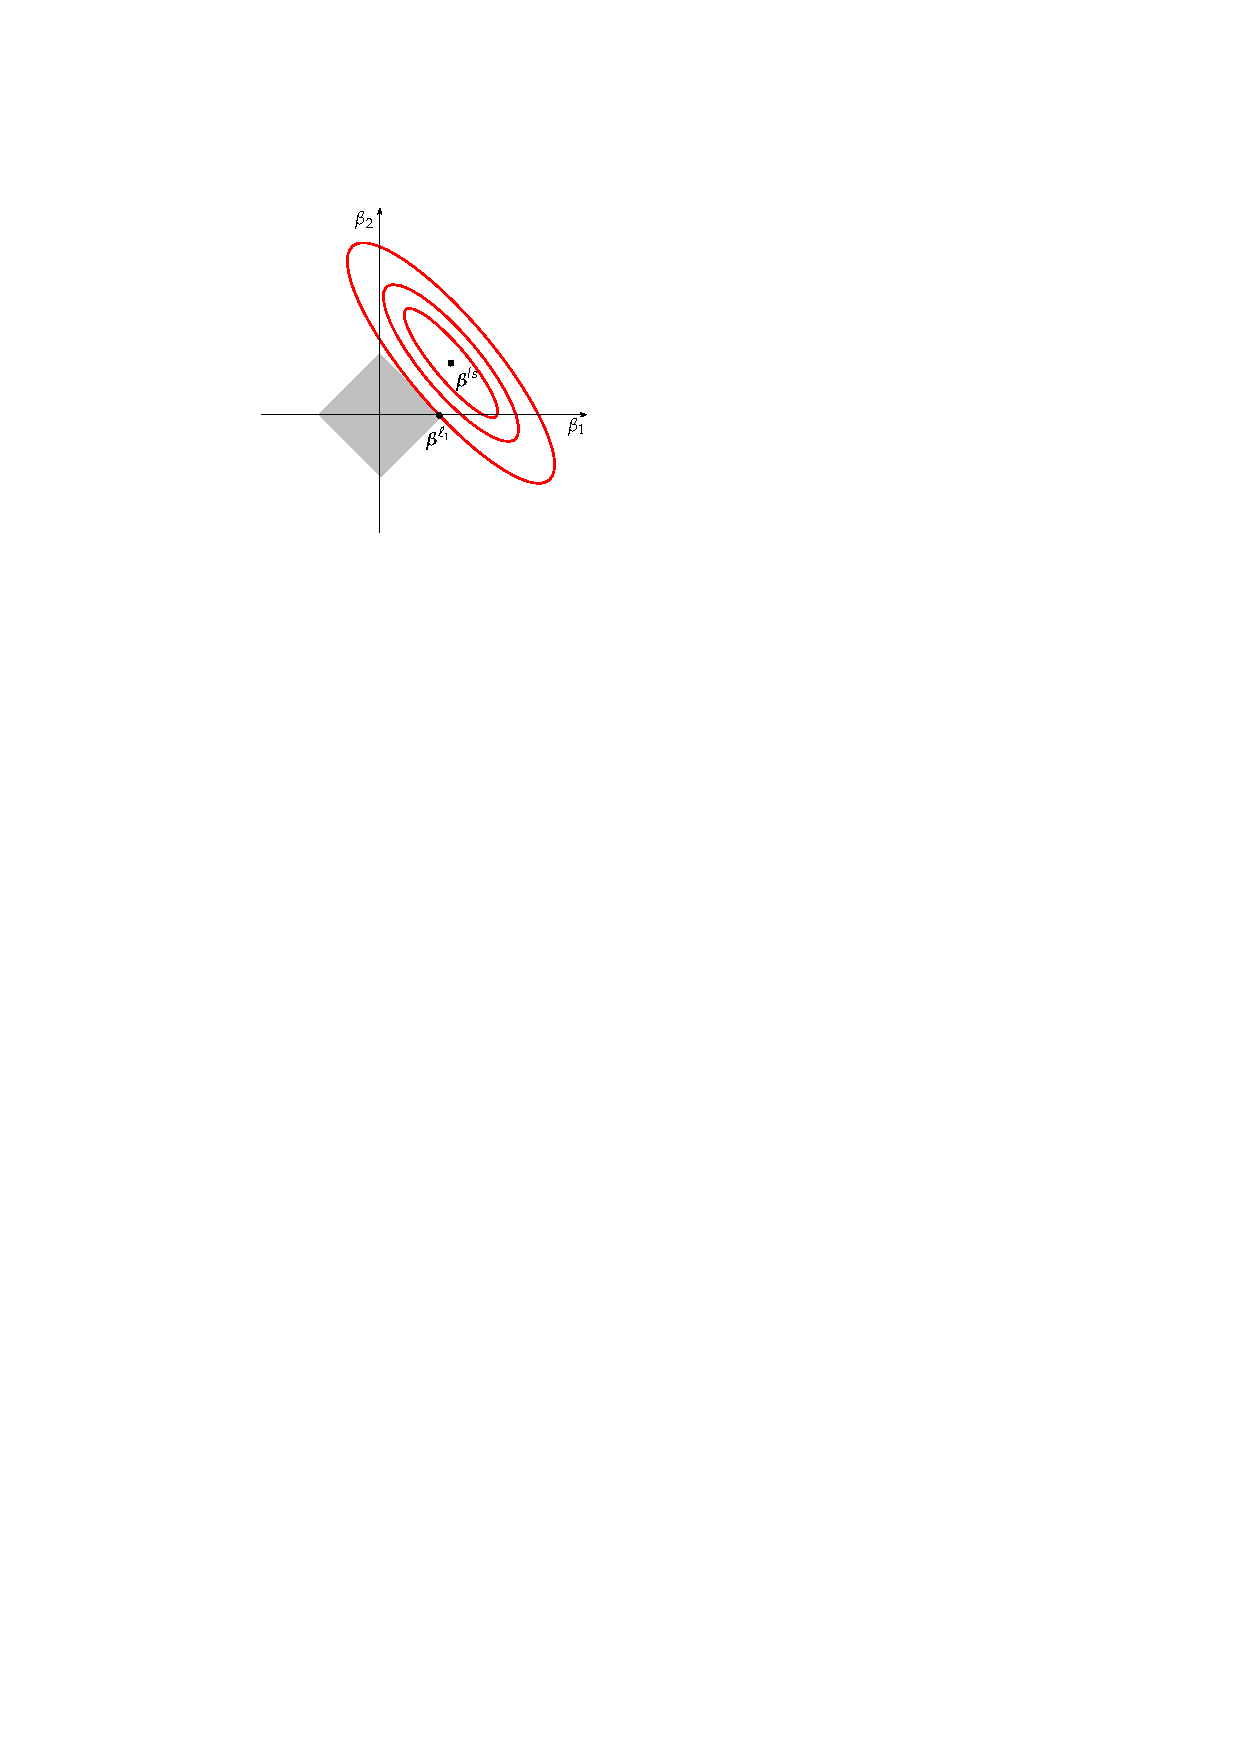
\includegraphics[width=.75\textwidth]{figures/lasso_set}
      \end{column}
    \end{columns}
  \end{overlayarea}

\end{frame}

\begin{frame}
  \frametitle{Insights: 2-dimensional example with the square loss}

  \begin{overlayarea}{\textwidth}{\textheight}

    \begin{equation*}
      \sum_{i=1}^n (y_i-x_i^1\Omega_1 - x_i^2\Omega_2)^2, \qquad
      \only<1>{\text{no constraints}}
      \only<2>{\text{s.t. } |\Omega_1| + |\Omega_2| < 0.75}
      \only<3>{\text{s.t. } |\Omega_1| + |\Omega_2| < 0.66}
      \only<4>{\text{s.t. } |\Omega_1| + |\Omega_2| < 0.4}
      \only<5>{\text{s.t. } |\Omega_1| + |\Omega_2| < 0.2}
      \only<6>{\text{s.t. } |\Omega_1| + |\Omega_2| < 0.0743}
    \end{equation*}

  \vspace{-.5cm}

    \includegraphics<1>[width=.8\textwidth]{dess11}
    \includegraphics<2>[width=.8\textwidth]{dess12}
    \includegraphics<3>[width=.8\textwidth]{dess13}
    \includegraphics<4>[width=.8\textwidth]{dess14}
    \includegraphics<5>[width=.8\textwidth]{dess15}
    \includegraphics<6>[width=.8\textwidth]{dess16}

  \end{overlayarea}

\end{frame}

\begin{frame}
  \frametitle{Application to GGM}

  \begin{block}{A penalized likelihood approach}
    \vspace{-1em}
    \begin{equation*}
      \hat{\bTheta}_\lambda=\argmax_{\bTheta \in \mathbb{S}_+}
      \ell(\bTheta;\mathbf{X})-\lambda
      \mathrm{pen}_{\ell_1}(\bTheta)
    \end{equation*}
  where
  \begin{itemize}
  \item $\mathcal{\ell}$ is the model log-likelihood,
  \item $\mathrm{pen}_{\ell_1}$ is a \alert{penalty function} tuned by
    $\lambda>0$.
    \vfill
      \begin{enumerate}
      \item \textit{regularization} (needed when $n \ll p$),
      \item \textit{selection} (sparsity induced by the $\ell_1$-norm).
      \end{enumerate}
  \end{itemize}
\end{block}

\end{frame}

\begin{frame}
  \frametitle{Gold standard penalized approaches}

  \vspace{-.25cm}
  
  \begin{overlayarea}{\textwidth}{\textheight}

    \begin{block}{Penalized   likelihood  (Banerjee   \textit{et
          al.}, Yuan and Lin, 2008)}
      \vspace{-1em}
      \begin{equation*}
        \hat{\bTheta}_\lambda=\argmax_{\bTheta \in \mathbb{S}_+}
        \ell(\bTheta;\mathbf{X})-\lambda
        \|\bTheta\|_{1}
      \end{equation*}
    \end{block}
    \vspace*{-1.5em}
    
    \begin{itemize}
    \item[\textcolor{green}{$+$}] symmetric, positive-definite
    \item[\textcolor{red}{$-$}]       solved      by       the
      ``Graphical-Lasso''                 ($\mathcal{O}(p^3)$,
      \textit{Friedman et al, 2007}).
    \item \texttt{R}-packages \textbf{glasso}, \textbf{quic}, \textbf{huge}.
    \end{itemize}
    
    \vfill
    
    \begin{block}{Neighborhood    Selection   (Meinshausen    \&
        B\"ulhman, 2006)}<2-> \vspace*{-1em}
      \only<2>{
         \begin{equation*}
          \text{For variable $j$, solve} \quad \hatbbeta_j  = \argmin_{\bbeta\in\Rset^{p-1}}
           \frac{1}{2} \|\bX_j - \bX_{\backslash j} \bbeta \|_2^2  + \lambda \|\bbeta\|_{\ell_1}.
          \end{equation*}
      }
      \only<3->{
      \begin{equation*}
        \hat{\mathbf{B}}^{\text{ns}}  = \argmin_{\mathbf{B}\in\Rset^{p\times  p}, \mathrm{diag}(\mathbf{B})
          = {\boldsymbol 0}_p} \frac{1}{2} \mathrm{tr}(\mathbf{B}^\top\mathbf{S}_n \mathbf{B}) -
        \mathrm{tr}(\mathbf{B}^\top\mathbf{S}_n) + \lambda \|\mathbf{B}\|_{\ell_1}.
      \end{equation*}
      }
      \vspace*{-1.5em}
    \end{block}
    
    \onslide<2->{
      \begin{itemize}
      \item[\textcolor{red}{$-$}]     not     symmetric,     not
        positive-definite
      \item[\textcolor{green}{$+$}]   $p$   Lasso  solved   with
        Lars-like   algorithms   ($\mathcal{O}(npd)$   for   $d$
        neighbors).
      \item \texttt{R}-package \textbf{huge}.
      \end{itemize}
    }
     
\end{overlayarea}      

\end{frame}

\subsection{Limitations and extensions of sparse GGM}

\begin{frame}
  \frametitle{Practical implications of theoretical results}

  \begin{block}{Selection    consistency    (Ravikumar,    Wainwright,
      2009-2012)}<1->                                           Denote
    $d=\max_{j\in\mathcal{P}}(\mathrm{degree_j})$.  Consistency for an
    appropriate $\lambda$ and
    \begin{itemize}
    \item  $n\approx\mathcal{O}(d^2\log(p))$ for  the graphical  Lasso
      and Clime.
    \item $n\approx\mathcal{O}(d\log(p))$  for   neighborhood
      selection (sharp).
    \end{itemize}
    \textit{(Irrepresentability) conditions are not strictly
    comparable\dots}
  \end{block}

  \vfill

  \begin{block}{Ultra high-dimension phenomenon (Verzelen,  2011)}<2>
    Minimax risk for sparse regression with $d$-sparse models: useless
    when
    \begin{equation*}
    \frac{d \log(p/d)}{n} \geq 1/2, \qquad (\mathrm{e.g.}, n=50, p=200, d\geq 8).
    \end{equation*}
    \textit{Good news! when $n$ is small, we don't need to solve
      huge problems because they can't but fail.}
  \end{block}

\end{frame}

\begin{frame}
  \frametitle{Model selection}

  \begin{block}{Cross-validation}
    Optimal in terms of \alert{prediction}, not in terms of selection
  \end{block}

  \begin{block}{Information based criteria}
    \begin{itemize}
    \item GGMSelect (Girault \textit{et al}, '12) selects among a family of candidates.
    \item Adapt IC to sparse high dimensional problems, e.g.
    \begin{equation*}
      \text{EBIC}_\gamma(\widehat{{\boldsymbol\Omega}}_\lambda)  =   -2 \textrm{loglik}
      (\widehat{{\boldsymbol\Omega}}_\lambda;\bX) + |\mathcal{E}_\lambda| (\log(n) + 4 \gamma \log(p) ),
    \end{equation*}
    \end{itemize}
  \end{block}

  \begin{block}{Resampling/subsampling}
    \alert{Keep edges frequently selected} on an range of $\lambda$ after sub-samplings
    \begin{itemize}
    \item Stability Selection (Meinshausen and B\"uhlman, 2010, Bach 2008)
    \item Stability approach to Regularization Selection (StaRS) (Liu, 2010).
    \end{itemize}
  \end{block}
\end{frame}

\subsection{Example: plasmodium data set}



\begin{frame}[fragile]
\frametitle{The plasmodium data}

\begin{knitrout}\scriptsize
\definecolor{shadecolor}{rgb}{0.969, 0.969, 0.969}\color{fgcolor}\begin{kframe}
\begin{alltt}
\hlkwd{library}\hlstd{(Matrix)}
\hlkwd{load}\hlstd{(}\hlstr{"plasmodium_expression.Rdata"}\hlstd{)}
\hlkwd{dim}\hlstd{(Y)}
\end{alltt}
\begin{verbatim}
## [1] 3490   46
\end{verbatim}
\begin{alltt}
\hlkwd{head}\hlstd{(Y)[,} \hlnum{1}\hlopt{:}\hlnum{5}\hlstd{]}
\end{alltt}
\begin{verbatim}
##                TP1    TP2    TP3    TP4    TP5
## MAL13P1.100 0.4510 0.6532 1.0760 0.5515 0.4238
## MAL13P1.102 1.5320 1.8920 0.8803 1.0300 0.9328
## MAL13P1.103 0.5218 0.5213 0.5328 0.3719 0.3258
## MAL13P1.105 0.5515 0.5527 0.8627 0.4541 0.4299
## MAL13P1.107 0.5630 0.4463 1.0760 0.4035 0.2082
## MAL13P1.112 0.5390 0.5393 0.5642 0.5326 0.4469
\end{verbatim}
\end{kframe}
\end{knitrout}
\end{frame}

\begin{frame}[fragile]
\frametitle{The plasmodium data}
\framesubtitle{Gene to Gene empirical covariance}

Covariance between the 100 most variable genes.

\begin{knitrout}\scriptsize
\definecolor{shadecolor}{rgb}{0.969, 0.969, 0.969}\color{fgcolor}\begin{kframe}
\begin{alltt}
\hlstd{genes.subset} \hlkwb{<-} \hlkwd{order}\hlstd{(}\hlkwd{apply}\hlstd{(Y,}\hlnum{1}\hlstd{,var))[}\hlnum{1}\hlopt{:}\hlnum{100}\hlstd{]}
\hlkwd{image}\hlstd{(}\hlkwd{Matrix}\hlstd{(}\hlkwd{cor}\hlstd{(}\hlkwd{t}\hlstd{(Y[genes.subset, ]))),} \hlkwc{userRaster}\hlstd{=}\hlnum{TRUE}\hlstd{)}
\end{alltt}
\end{kframe}
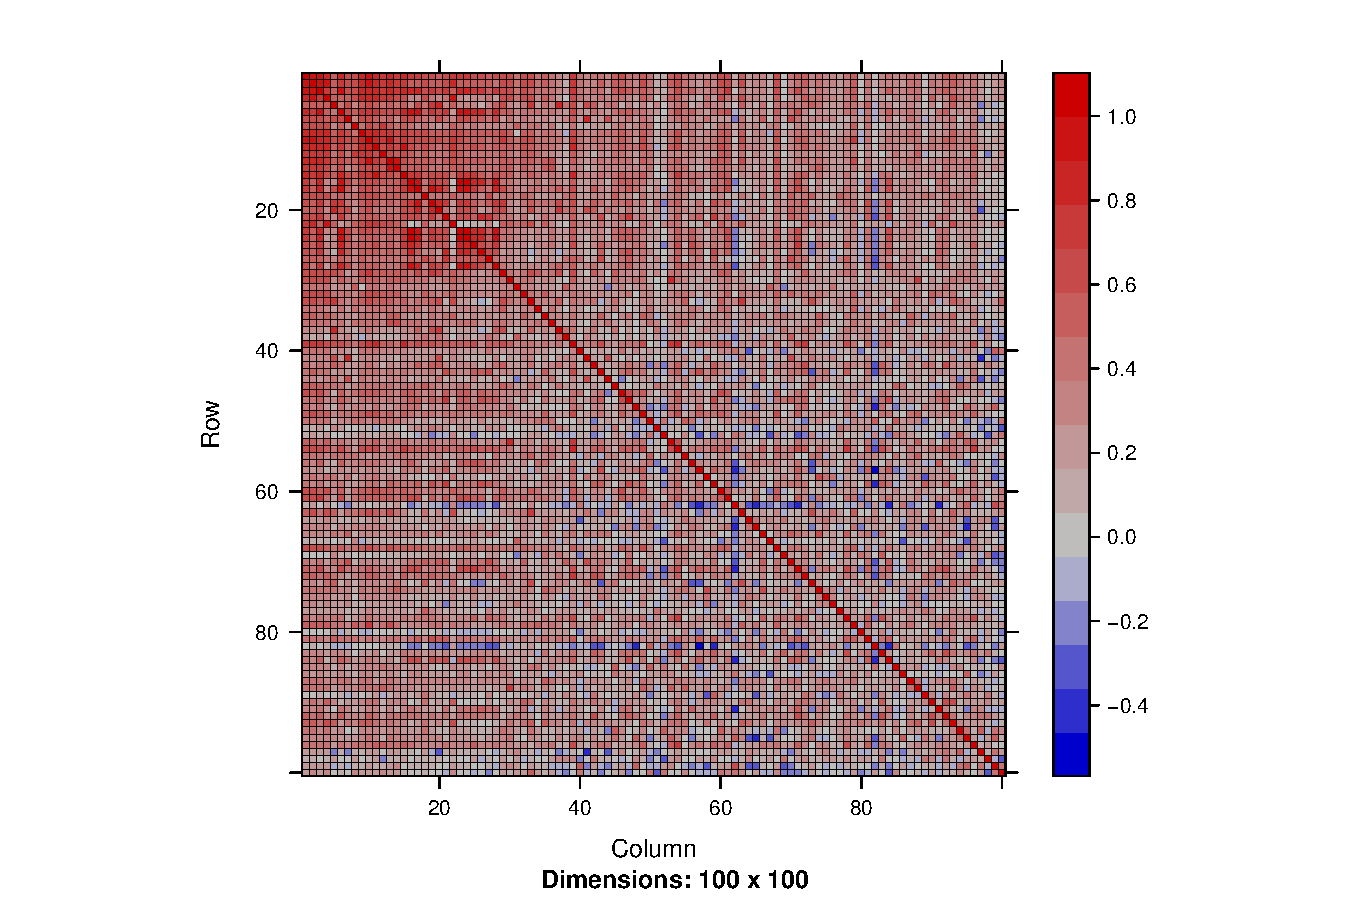
\includegraphics[width=.8\textwidth]{figures/get_plasmodium_data_fig-1} 

\end{knitrout}
\end{frame}

\begin{frame}[containsverbatim,allowframebreaks]
\frametitle{Network between the genes}
\framesubtitle{Sparse Estimation}

Regulatory network between the 100 most variable genes.

\begin{knitrout}\scriptsize
\definecolor{shadecolor}{rgb}{0.969, 0.969, 0.969}\color{fgcolor}\begin{kframe}
\begin{alltt}
\hlkwd{library}\hlstd{(huge)}
\hlstd{huge.out} \hlkwb{<-} \hlkwd{huge}\hlstd{(}\hlkwd{as.matrix}\hlstd{(}\hlkwd{t}\hlstd{(Y[genes.subset, ])),} \hlkwc{method}\hlstd{=}\hlstr{"glasso"}\hlstd{,} \hlkwc{cov.output}\hlstd{=}\hlnum{TRUE}\hlstd{)}
\end{alltt}
\begin{verbatim}
## Conducting the graphical lasso (glasso) with lossless screening....in progress:0% 
Conducting the graphical lasso (glasso) with lossless screening....in progress:9% 
Conducting the graphical lasso (glasso) with lossless screening....in progress:19% 
Conducting the graphical lasso (glasso) with lossless screening....in progress:30% 
Conducting the graphical lasso (glasso) with lossless screening....in progress:40% 
Conducting the graphical lasso (glasso) with lossless screening....in progress:50% 
Conducting the graphical lasso (glasso) with lossless screening....in progress:60% 
Conducting the graphical lasso (glasso) with lossless screening....in progress:70% 
Conducting the graphical lasso (glasso) with lossless screening....in progress:80% 
Conducting the graphical lasso (glasso)....done.                                          
\end{verbatim}
\begin{alltt}
\hlkwd{plot}\hlstd{(huge.out)}
\end{alltt}
\end{kframe}
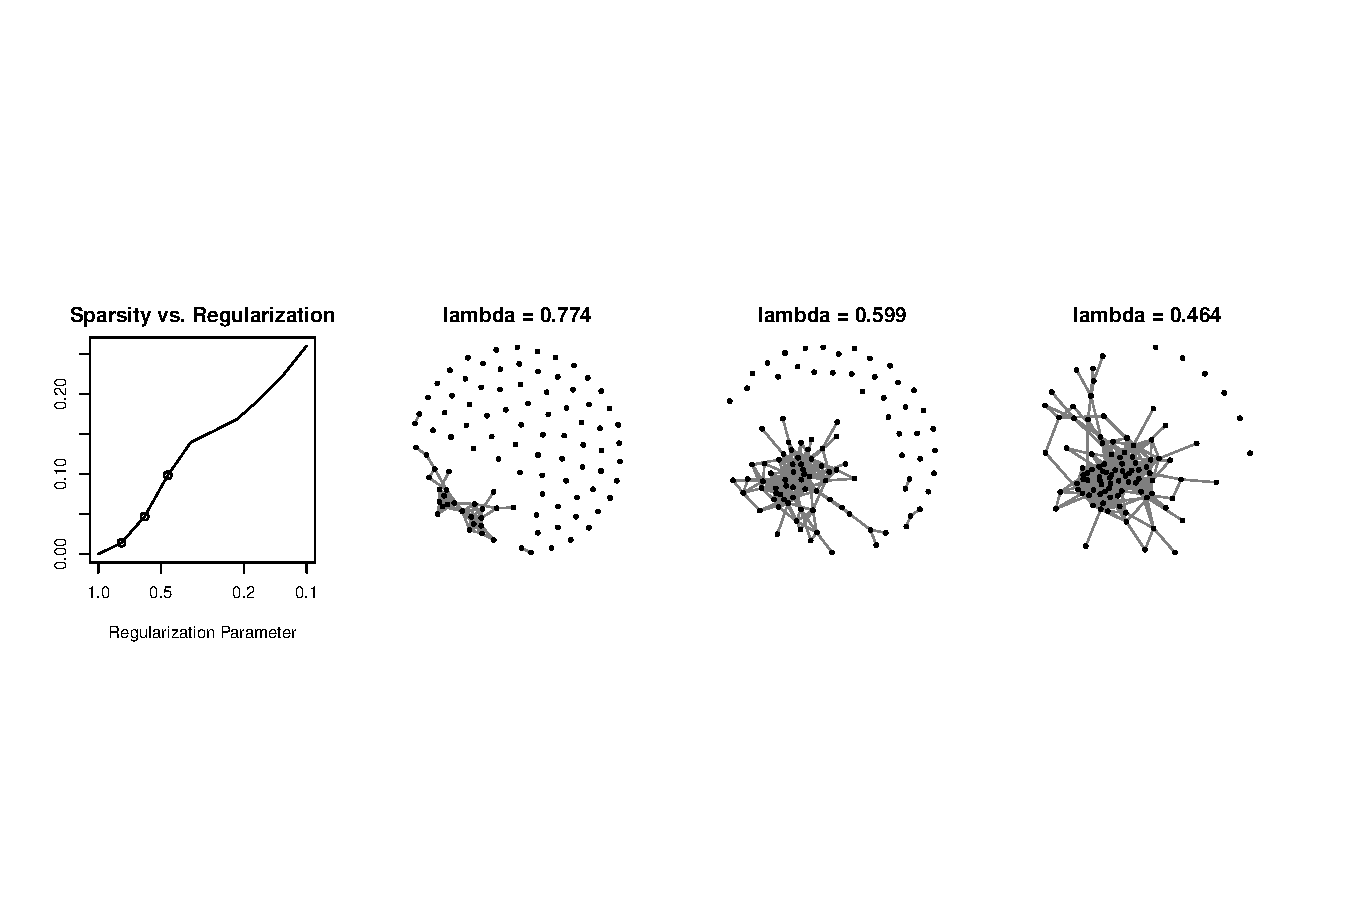
\includegraphics[width=.8\textwidth]{figures/r_show_plasmodium_glasso3-1} 

\end{knitrout}
\end{frame}

\begin{frame}[containsverbatim,allowframebreaks]
\frametitle{Network between the genes}
\framesubtitle{Inverse covariance}

\begin{knitrout}\scriptsize
\definecolor{shadecolor}{rgb}{0.969, 0.969, 0.969}\color{fgcolor}\begin{kframe}
\begin{alltt}
\hlkwd{library}\hlstd{(huge)}
\hlstd{huge.out}\hlopt{$}\hlstd{df}
\end{alltt}
\begin{verbatim}
##  [1]    0   71  233  488  693  763  836  963 1110 1289
\end{verbatim}
\begin{alltt}
\hlkwd{image}\hlstd{(}\hlkwd{Matrix}\hlstd{(huge.out}\hlopt{$}\hlstd{icov[[}\hlnum{3}\hlstd{]]))}
\end{alltt}
\end{kframe}
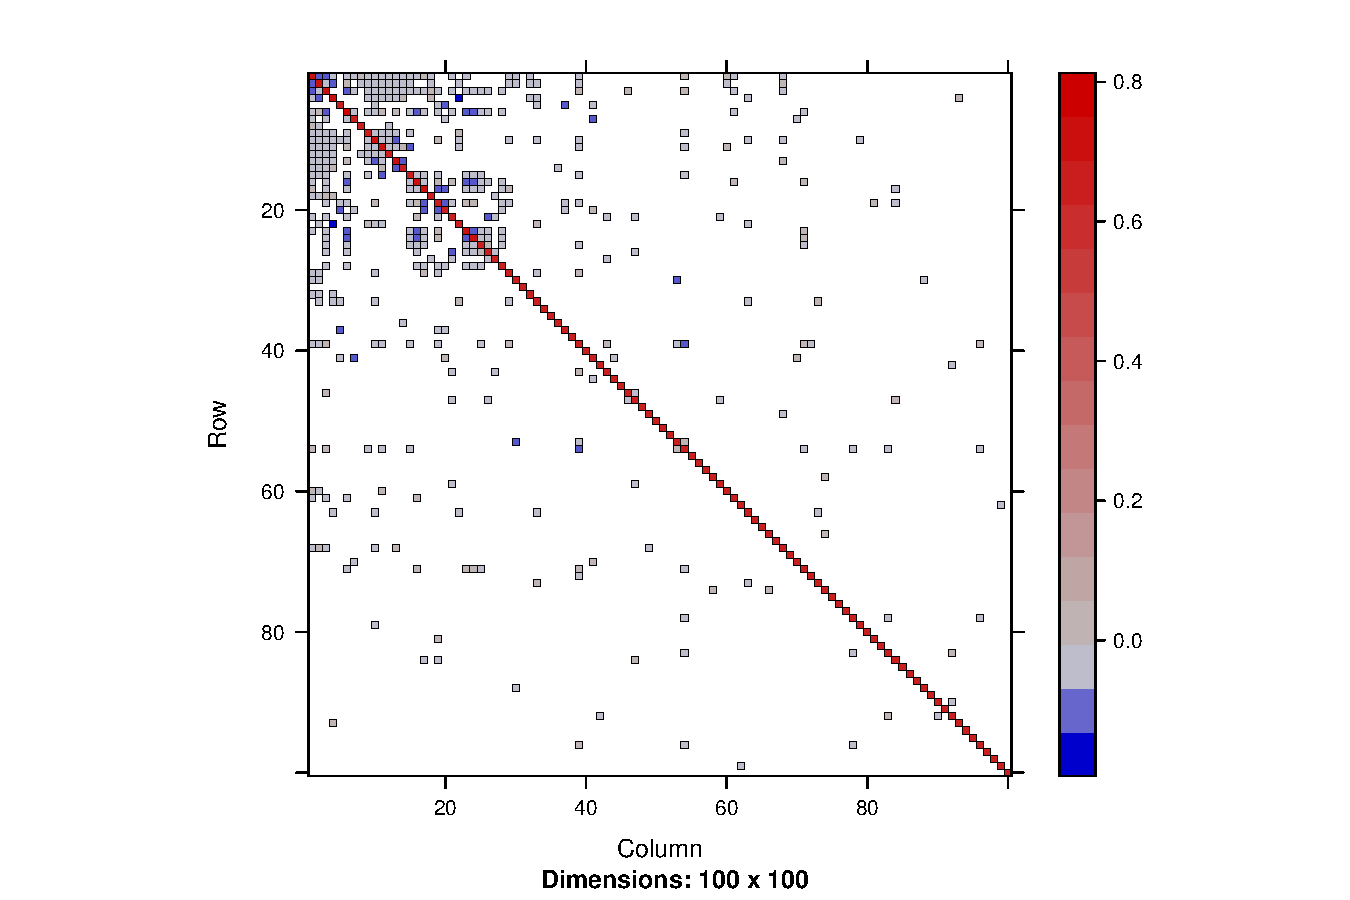
\includegraphics[width=.8\textwidth]{figures/r_show_plasmodium_glasso4-1} 

\end{knitrout}
\end{frame}

\begin{frame}[fragile]
\frametitle{The plasmodium data}
\framesubtitle{Covariance between conditions}

\begin{knitrout}\scriptsize
\definecolor{shadecolor}{rgb}{0.969, 0.969, 0.969}\color{fgcolor}\begin{kframe}
\begin{alltt}
\hlkwd{image}\hlstd{(}\hlkwd{Matrix}\hlstd{(}\hlkwd{cor}\hlstd{(Y)))}
\end{alltt}
\end{kframe}
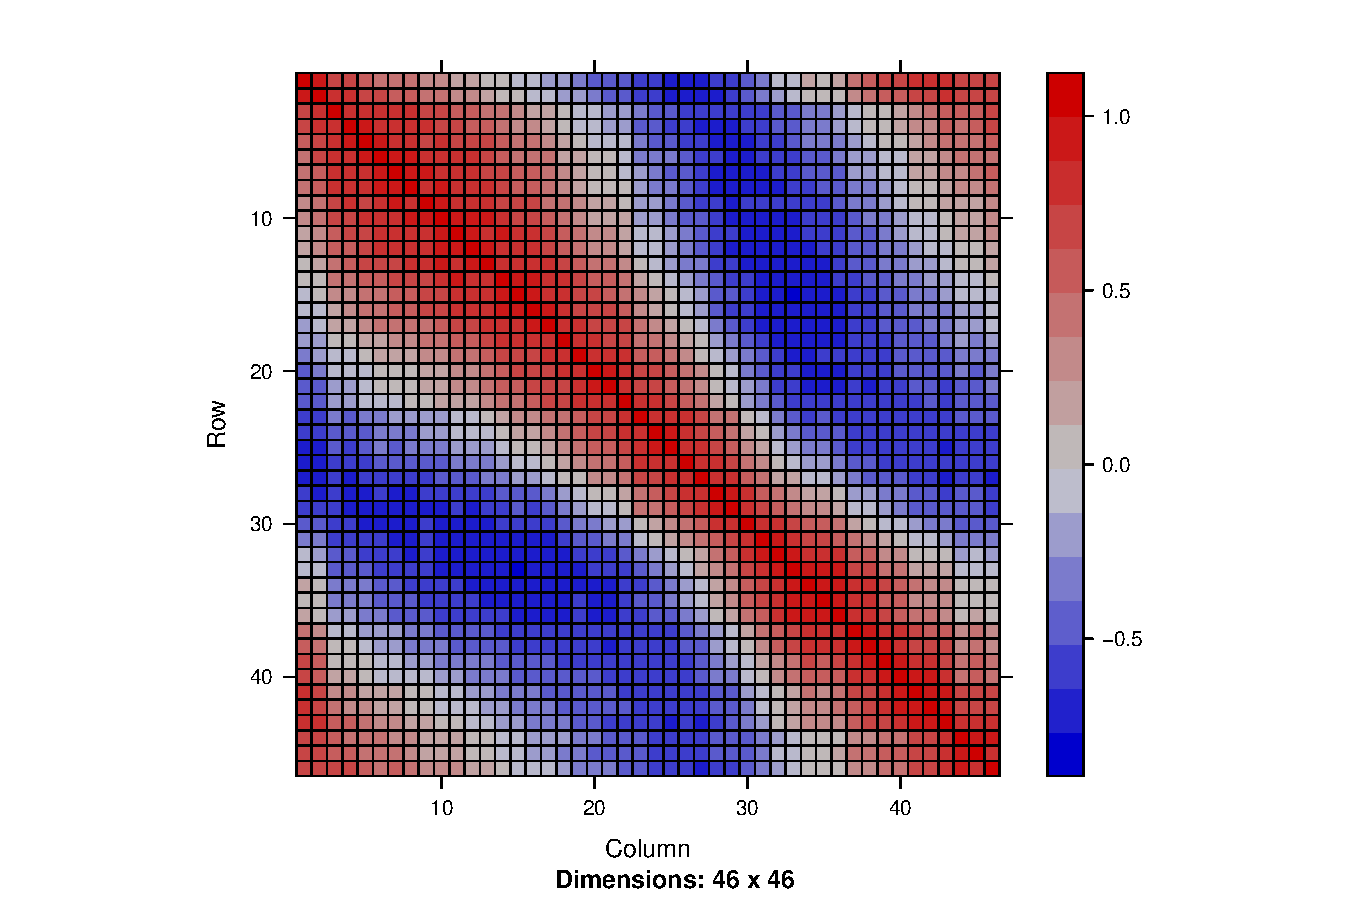
\includegraphics[width=.8\textwidth]{figures/get_plasmodium_data_fig_cond-1} 

\end{knitrout}
\end{frame}

\begin{frame}[containsverbatim]
\frametitle{Covariance structure between the conditions}
\framesubtitle{Sparse Estimation}

\begin{knitrout}\scriptsize
\definecolor{shadecolor}{rgb}{0.969, 0.969, 0.969}\color{fgcolor}\begin{kframe}
\begin{alltt}
\hlkwd{library}\hlstd{(huge)}
\hlstd{huge.out} \hlkwb{<-} \hlkwd{huge}\hlstd{(}\hlkwd{as.matrix}\hlstd{(Y),} \hlkwc{method}\hlstd{=}\hlstr{"glasso"}\hlstd{,} \hlkwc{cov.output}\hlstd{=}\hlnum{TRUE}\hlstd{)}
\end{alltt}
\begin{verbatim}
## Conducting the graphical lasso (glasso) with lossless screening....in progress:0% 
Conducting the graphical lasso (glasso) with lossless screening....in progress:9% 
Conducting the graphical lasso (glasso) with lossless screening....in progress:19% 
Conducting the graphical lasso (glasso) with lossless screening....in progress:30% 
Conducting the graphical lasso (glasso) with lossless screening....in progress:40% 
Conducting the graphical lasso (glasso) with lossless screening....in progress:50% 
Conducting the graphical lasso (glasso) with lossless screening....in progress:60% 
Conducting the graphical lasso (glasso) with lossless screening....in progress:70% 
Conducting the graphical lasso (glasso) with lossless screening....in progress:80% 
Conducting the graphical lasso (glasso)....done.                                          
\end{verbatim}
\begin{alltt}
\hlstd{sel.out}  \hlkwb{<-} \hlkwd{huge.select}\hlstd{(huge.out)}
\end{alltt}
\begin{verbatim}
## Conducting extended Bayesian information criterion (ebic) selection....done
\end{verbatim}
\end{kframe}
\end{knitrout}
\end{frame}

\begin{frame}[containsverbatim]
\frametitle{Covariance structure between the conditions}
\framesubtitle{Sparse Estimation}

\begin{knitrout}\scriptsize
\definecolor{shadecolor}{rgb}{0.969, 0.969, 0.969}\color{fgcolor}\begin{kframe}
\begin{alltt}
\hlkwd{image}\hlstd{(sel.out}\hlopt{$}\hlstd{opt.cov)}
\end{alltt}
\end{kframe}
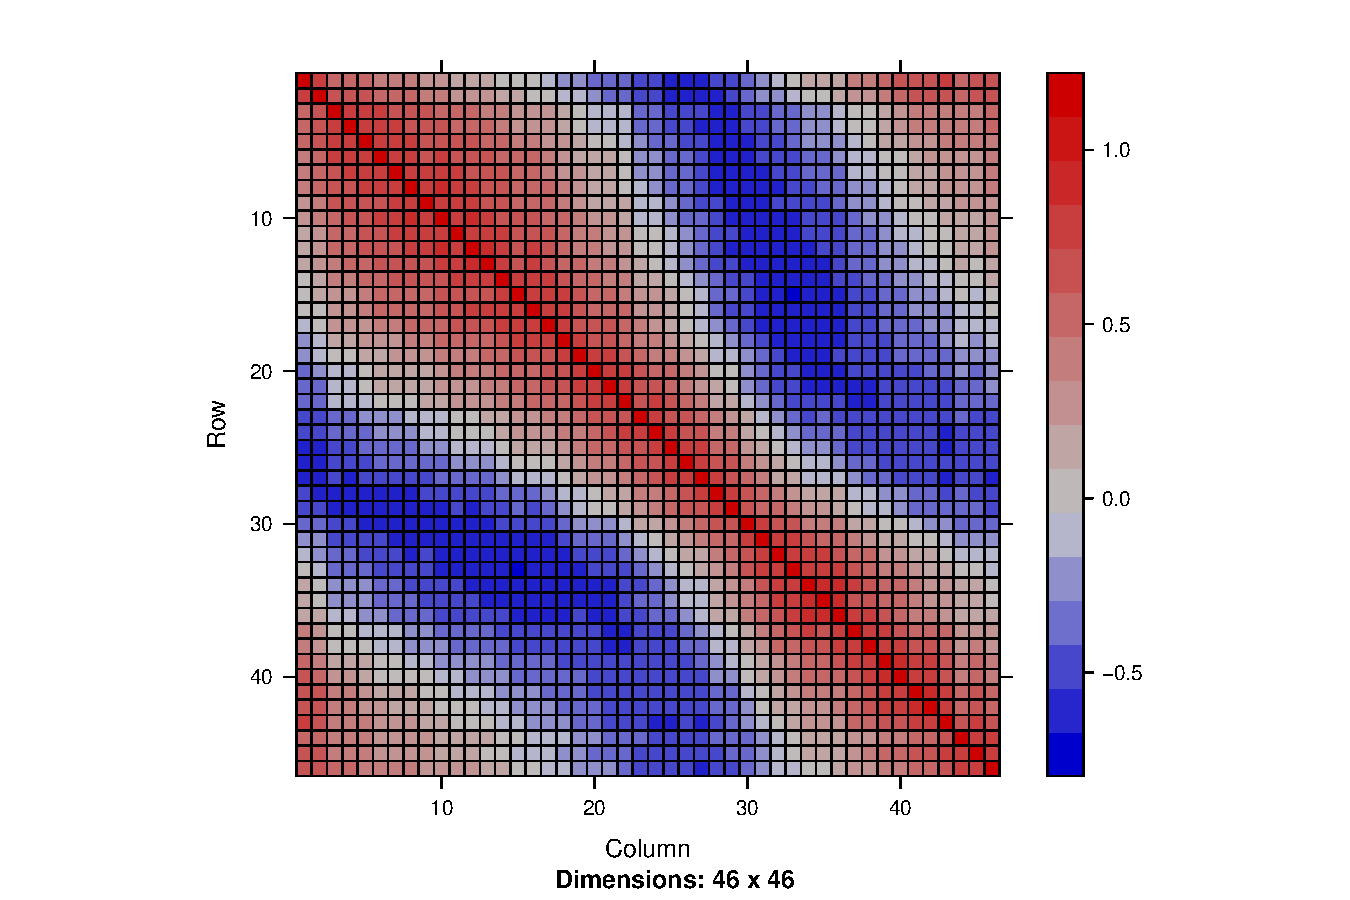
\includegraphics[width=.8\textwidth]{figures/r_get_plasmodium_glassob-1} 

\end{knitrout}
\end{frame}

\begin{frame}[containsverbatim,allowframebreaks]
\frametitle{Covariance structure between the conditions}
\framesubtitle{Sparse Estimation of the inverse covariance}

\begin{knitrout}\scriptsize
\definecolor{shadecolor}{rgb}{0.969, 0.969, 0.969}\color{fgcolor}\begin{kframe}
\begin{alltt}
\hlkwd{sum}\hlstd{(}\hlkwd{abs}\hlstd{(sel.out}\hlopt{$}\hlstd{opt.icov)} \hlopt{!=} \hlnum{0}\hlstd{)}
\end{alltt}
\begin{verbatim}
## [1] 760
\end{verbatim}
\begin{alltt}
\hlkwd{ncol}\hlstd{(sel.out}\hlopt{$}\hlstd{opt.icov)} \hlopt{**} \hlnum{2}
\end{alltt}
\begin{verbatim}
## [1] 2116
\end{verbatim}
\begin{alltt}
\hlkwd{image}\hlstd{(sel.out}\hlopt{$}\hlstd{opt.icov)}
\end{alltt}
\end{kframe}
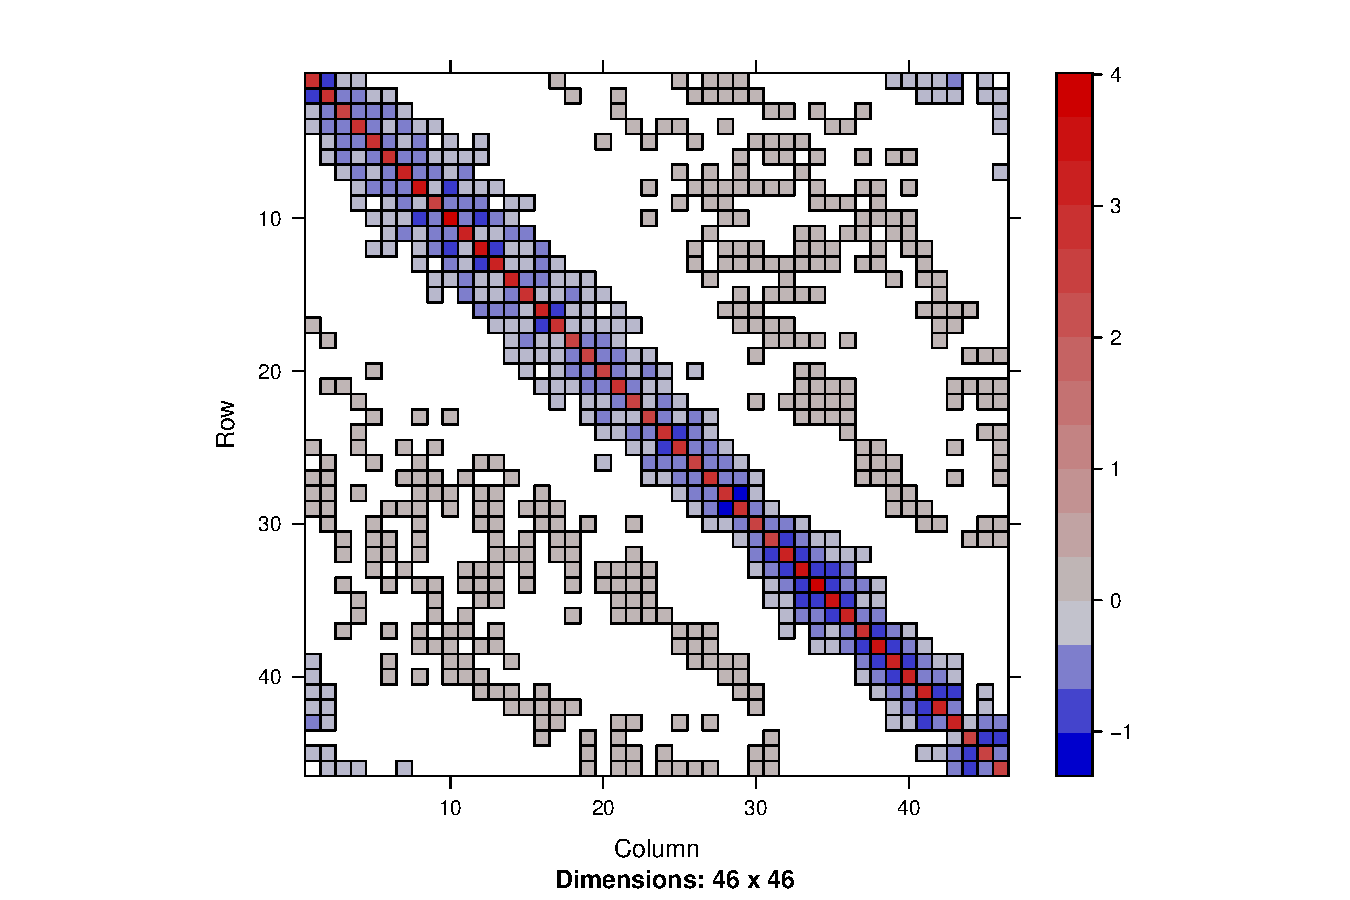
\includegraphics[width=.8\textwidth]{figures/r_show_plasmodium_glasso-1} 

\end{knitrout}

\end{frame}

\begin{frame}[containsverbatim,allowframebreaks]
\frametitle{Covariance structure between the conditions}
\framesubtitle{Associated network}

\begin{knitrout}\scriptsize
\definecolor{shadecolor}{rgb}{0.969, 0.969, 0.969}\color{fgcolor}\begin{kframe}
\begin{alltt}
\hlkwd{plot}\hlstd{(huge.out)}
\end{alltt}
\end{kframe}
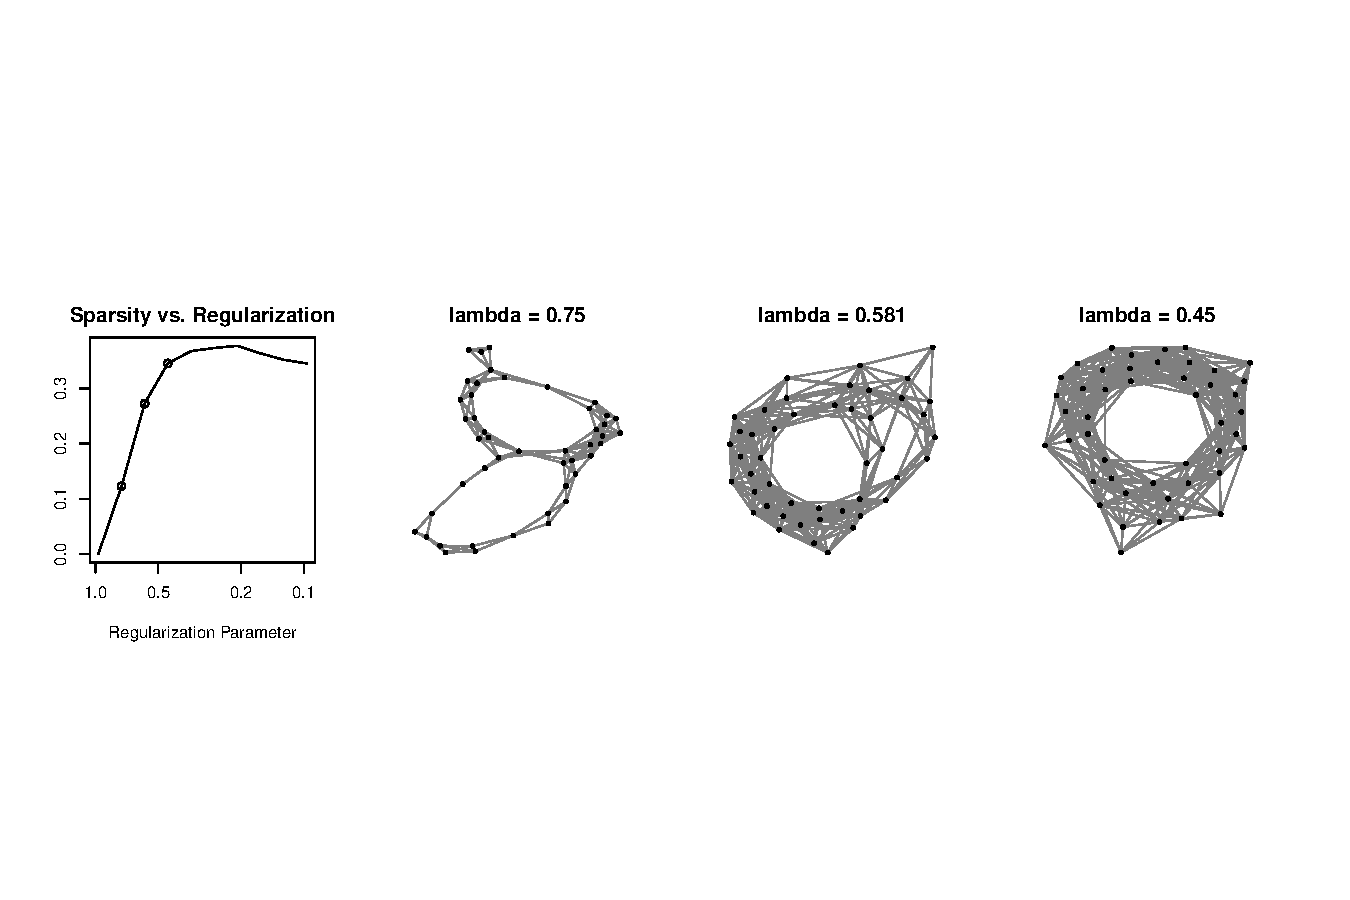
\includegraphics[width=.8\textwidth]{figures/r_show_plasmodium_glasso2-1} 

\end{knitrout}

\end{frame}




\section{Network inference with GGM}

\begin{frame}
  \frametitle{Some families of methods for network reconstruction}

  \begin{block}{Test-based methods}
    \begin{itemize}
    \item Tests the nullity of each entries 
    \item Combinatorial problem when $p>30$ \dots
    \end{itemize}    
  \end{block}
  
  \vfill

  \begin{block}{\alert{Sparsity-inducing regularization methods}}
    \begin{itemize}
    \item induce sparsity with the $\ell_1$-norm penalization
    \item Use results from convex optimization
    \item Versatile and computationally efficient
    \end{itemize}
  \end{block}

  \vfill

  \begin{block}{Bayesian methods}
    \begin{itemize}
    \item Compute the posterior probability of each edge
    \item Usually more computationally demanding
    \item For special graphs, computation gets easier
    \end{itemize}
  \end{block}
  
\end{frame}

\subsection{Inducing sparsity for edge selection}

\begin{frame}
  \frametitle{Inference: maximum likelihood estimator}
  \framesubtitle{The natural approach for parametric statistics}
  
  Let   $X$  be  a   random  vector   with  distribution   defined  by
  $f_{X}(x;\boldsymbol\Theta)$,  where   $\boldsymbol\Theta$  are  the
  model parameters.

  \vfill

  \begin{block}{Maximum likelihood estimator}
    \begin{equation*}
      \hat{\boldsymbol\Theta}      =      \argmax_{\boldsymbol\Theta}
      \ell(\boldsymbol\Theta; \mathbf{X})
    \end{equation*} 
    where  $\ell$ is  the log  likelihood, a  function  of the
    parameters:
    \begin{equation*}
      \ell(\boldsymbol\Theta;      \mathbf{X})      =     \log
      \prod_{i=1}^n f_{X}(\mathbf{x}_i;\boldsymbol\Theta),
    \end{equation*}
    where $\mathbf{x}_i$ is the $i$th row of $\mathbf{X}$.
  \end{block}
  
  \vfill
  
  \begin{block}{Remarks}
    \begin{itemize}
    \item This a convex optimization problem,
    \item We just need to detect non zero coefficients in $\boldsymbol\Theta$
    \end{itemize}
  \end{block}
  
\end{frame}

\begin{frame}
  \frametitle{The multivariate Gaussian log-likelihood }
  
  Let  $\mathbf{S}  =  n^{-1}\mathbf{X}^\intercal \mathbf{X}$  be  the
  empirical variance-covariance  matrix: $\mathbf{S}$ is  a sufficient
  statistic of $ \boldsymbol\Theta$.

  \vfill

  \begin{block}{The log-likelihood}
    \begin{equation*}
      \ell(\boldsymbol\Theta; \mathbf{S}) =
      \frac{n}{2}     \log    \det     (\boldsymbol\Theta)  - \frac{n}{2}
      \mathrm{Trace}(\mathbf{S} \boldsymbol\Theta) + \frac{n}{2}\log(2\pi).
    \end{equation*}
  \end{block}
  
  \vfill
  
  \begin{itemize}
  \item[$\rightsquigarrow$]    The     MLE    $=\mathbf{S}^{-1}$    of
    $\boldsymbol\Theta$ is not defined for $n< p$ and never sparse.
  \item[$\rightsquigarrow$] The need for regularization is huge.
  \end{itemize}
\end{frame}

\begin{frame}
  \frametitle{Application to GGM: the "Graphical-Lasso"} 

  \begin{block}{A penalized likelihood approach}
    \vspace{-1em}
    \begin{equation*}
      \hat{\bTheta}_\lambda=\argmax_{\bTheta \in \mathbb{S}_+}
      \ell(\bTheta;\mathbf{X})-\lambda
      \|\bTheta\|_{\ell_1}
    \end{equation*}
  where
  \begin{itemize}
  \item $\mathcal{\ell}$ is the model log-likelihood,
  \item $\|\cdot\|_{\ell_1}$ is a \alert{penalty function} tuned by
    $\lambda>0$. 
    \vfill
      \begin{enumerate}
      \item \textit{regularization} (needed when $n \ll p$), 
      \item \textit{selection} (sparsity induced by the $\ell_1$-norm),
      \end{enumerate}
    \item     solved    in     \texttt{R}-packages    \textbf{glasso},
      \textbf{quic}, \textbf{huge} ($\mathcal{O}(p^3)$)
  \end{itemize}
\end{block}

\end{frame}

\begin{frame}
  \frametitle{Application to GGM: "Neighborhood selection"} 

  A close cousin, thank to the relationship between Gaussian vector and linear regression
  
  \textcolor{gray}{
  Remember that
  \begin{equation*}
    X_i | X_{ \setminus i} = \sum_{\alert{j \in \text{neighbors}(i)}} \beta_j X_j + \varepsilon_i
    \quad         \text{with         }         \beta_j         =
    -\frac{\Theta_{ij}}{\Theta_{ii}}.
  \end{equation*}
  }
  
  \begin{block}{A penalized least-square approach}
    Let $\bX_i$ be the $i$th column of the data matrix (i.e data associated to variable (gene) $i$), and $\bX_{\backslash i}$ deprived of colmun $i$. We select the neighbors of variable $i$ by solving
    \begin{equation*}
      \widehat{\boldsymbol\beta}^{(i)} = \argmin_{\boldsymbol\beta \in \mathbb{R}^{p-1} }
      \frac{1}{n} \left\| \mathbf{X}_i - \mathbf{X}_{\backslash i} \,
        {\boldsymbol\beta} \right\|_2^2 + \lambda \left\| {\boldsymbol\beta} \right\|_{1}
    \end{equation*}

    \begin{itemize}
    \item[\textcolor{red}{$-$}] not symmetric, not positive-definite
    \item[\textcolor{green}{$+$}] $p$
      Lasso solved with Lars-like algorithms ($\mathcal{O}(npd)$ for $d$ neighbors).
    \end{itemize}

\end{block}

\end{frame}



\subsection{Limitations of sparse GGM}

\begin{frame}
  \frametitle{Practical implications of theoretical results}

  \begin{block}{Selection    consistency    (Ravikumar,    Wainwright,
      2009-2012)}<1->                                           Denote
    $d=\max_{j\in\mathcal{P}}(\mathrm{degree_j})$.  Consistency for an
    appropriate $\lambda$ and
    \begin{itemize}
    \item  $n\approx\mathcal{O}(d^2\log(p))$ for  the graphical  Lasso
      and Clime.
    \item $n\approx\mathcal{O}(d\log(p))$  for   neighborhood
      selection (sharp).
    \end{itemize}
    \textit{(Irrepresentability) conditions are not strictly
    comparable\dots}
  \end{block}

  \vfill

  \begin{block}{Ultra high-dimension phenomenon (Verzelen,  2011)}<2>
    Minimax risk for sparse regression with $d$-sparse models: useless
    when
    \begin{equation*}
    \frac{d \log(p/d)}{n} \geq 1/2, \qquad (\mathrm{e.g.}, n=50, p=200, d\geq 8).
    \end{equation*}
    \textit{Good news! when $n$ is small, we don't need to solve
      huge problems because they can't but fail.}
  \end{block}

\end{frame}

\begin{frame}
  \frametitle{Model selection}
  
  \begin{block}{Cross-validation}
    Optimal in terms of \alert{prediction}, not in terms of selection
  \end{block}

  \begin{block}{Information based criteria}
    \begin{itemize}
    \item GGMSelect (Girault \textit{et al}, '12) selects among a family of candidates.
    \item Adapt IC to sparse high dimensional problems, e.g.
    \begin{equation*}
      \text{EBIC}_\gamma(\widehat{{\boldsymbol\Theta}}_\lambda)  =   -2 \textrm{loglik}
      (\widehat{{\boldsymbol\Theta}}_\lambda;\bX) + |\mathcal{E}_\lambda| (\log(n) + 4 \gamma \log(p) ),
    \end{equation*}
    \end{itemize}
  \end{block}

  \begin{block}{Resampling/subsampling}
    \alert{Keep edges frequently selected} on an range of $\lambda$ after sub-samplings
    \begin{itemize}
    \item Stability Selection (Meinshausen and B\"uhlman, 2010, Bach 2008)
    \item Stability approach to Regularization Selection (StaRS) (Liu, 2010).
    \end{itemize}
  \end{block}
\end{frame}

\begin{frame}
  \frametitle{Concluding remark about GGM}

    \begin{block}{Sparse GGM}
    \begin{itemize}
      \item[\textcolor{green}{$+$}]     very     solid
      \alert{statistical} and \alert{computational} framework
      \item[\textcolor{green}{$+$}] \alert{competitive}  to other inference
        methods (DREAM 5 benchmark, 2012)
      \item[\textcolor{red}{$-$}]        performances        remain
        \alert{questionable on real data}, as for other methods
      \end{itemize}
    \end{block}

    \rsa Network inference is a very difficult problem

    \rsa Some biological questions can be answered without network inference

\end{frame}


%% simple simu GGM

\section{A tour of the \texttt{huge} package assessing GGM approach}



\begin{frame}[fragile]
  \frametitle{Assess the standard GGMs approaches}

Full analysis can be found at \url{http://julien.cremeriefamily.info/doc/teachings/exposome/td_exposome_correction.html}

\begin{knitrout}\scriptsize
\definecolor{shadecolor}{rgb}{0.969, 0.969, 0.969}\color{fgcolor}\begin{kframe}
\begin{alltt}
\hlkwd{suppressMessages}\hlstd{(}\hlkwd{library}\hlstd{(huge,} \hlkwc{quietly} \hlstd{=} \hlnum{TRUE}\hlstd{))}
\end{alltt}
\end{kframe}
\end{knitrout}

\begin{enumerate}
\item Simulated data
\begin{itemize}
    \item Test that an approach is working under some simple conditions
    \item Especially usefull when the approach has no underlying model
    \item Essential sanity check
\end{itemize}
\item Breast cancer data (pinpoint interesting genes/pathways)
\begin{itemize}
    \item Several hundred breast cancers (estrogen receptor + and -)
    \item Several thousand genes 
    \item Goal: How can GGMs approaches help ? 
\end{itemize}
\end{enumerate}

\end{frame}

\begin{frame}[fragile]
  \frametitle{Simple simulations (network with hubs)}

\begin{knitrout}\scriptsize
\definecolor{shadecolor}{rgb}{0.969, 0.969, 0.969}\color{fgcolor}\begin{kframe}
\begin{alltt}
\hlkwd{set.seed}\hlstd{(}\hlnum{11}\hlstd{)}
\hlstd{n} \hlkwb{<-} \hlnum{80}\hlstd{; d} \hlkwb{<-} \hlnum{10}\hlstd{;}
\hlstd{rd.net}  \hlkwb{<-} \hlkwd{huge.generator}\hlstd{(}
  \hlstd{n,} \hlcom{## number of samples}
  \hlstd{d,} \hlcom{## number of genes}
  \hlkwc{graph}\hlstd{=}\hlstr{"hub"}\hlstd{,} \hlcom{## type of net}
  \hlkwc{g} \hlstd{=} \hlnum{2}\hlstd{,} \hlcom{## number of group)}
  \hlkwc{verbose}\hlstd{=}\hlnum{FALSE}\hlstd{)}
\end{alltt}
\end{kframe}
\end{knitrout}

\end{frame}

\begin{frame}[fragile]
  \frametitle{Simple simulations (network with hubs)}



\begin{knitrout}\scriptsize
\definecolor{shadecolor}{rgb}{0.969, 0.969, 0.969}\color{fgcolor}\begin{kframe}
\begin{alltt}
\hlkwd{plot}\hlstd{(rd.net)}
\end{alltt}
\end{kframe}
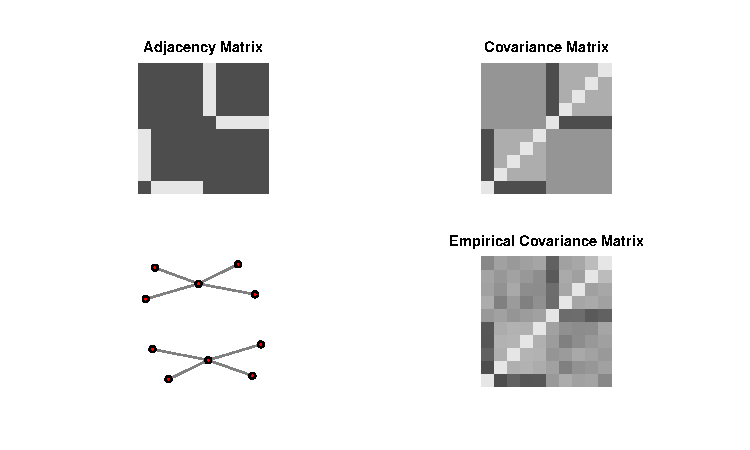
\includegraphics[width=.8\textwidth]{figures/r_simu_hub_plot-1} 

\end{knitrout}

\end{frame}

\begin{frame}[fragile]
  \frametitle{Inference using GGMs and correlation}

\paragraph{Inference}

\begin{knitrout}\scriptsize
\definecolor{shadecolor}{rgb}{0.969, 0.969, 0.969}\color{fgcolor}\begin{kframe}
\begin{alltt}
\hlcom{## glasso, mb and ct}
\hlstd{glasso} \hlkwb{<-} \hlkwd{huge}\hlstd{(rd.net}\hlopt{$}\hlstd{data,} \hlkwc{method}\hlstd{=}\hlstr{"glasso"}\hlstd{,}
               \hlkwc{nlambda}\hlstd{=}\hlnum{50}\hlstd{,}  \hlkwc{verbose}\hlstd{=F)}
\hlstd{mb} \hlkwb{<-} \hlkwd{huge}\hlstd{(rd.net}\hlopt{$}\hlstd{data,} \hlkwc{method}\hlstd{=}\hlstr{"mb"}\hlstd{,}
           \hlkwc{nlambda}\hlstd{=}\hlnum{50}\hlstd{,} \hlkwc{verbose}\hlstd{=F)}
\hlstd{corthr} \hlkwb{<-} \hlkwd{huge}\hlstd{(rd.net}\hlopt{$}\hlstd{data,} \hlkwc{method}\hlstd{=}\hlstr{"ct"}\hlstd{,}
              \hlkwc{nlambda} \hlstd{=} \hlnum{50}\hlstd{,} \hlkwc{verbose}\hlstd{=F)}
\end{alltt}
\end{kframe}
\end{knitrout}

\paragraph{Selection}

\begin{knitrout}\scriptsize
\definecolor{shadecolor}{rgb}{0.969, 0.969, 0.969}\color{fgcolor}\begin{kframe}
\begin{alltt}
\hlcom{## glasso, mb and ct}
\hlstd{glasso.sel} \hlkwb{<-} \hlkwd{huge.select}\hlstd{(glasso,} \hlstr{"stars"}\hlstd{,} \hlkwc{verbose}\hlstd{=F)}
\hlstd{mb.sel} \hlkwb{<-} \hlkwd{huge.select}\hlstd{(mb,} \hlstr{"stars"}\hlstd{,} \hlkwc{verbose}\hlstd{=F)}
\hlstd{corthr.sel} \hlkwb{<-} \hlkwd{huge.select}\hlstd{(corthr,} \hlstr{"stars"}\hlstd{,} \hlkwc{verbose}\hlstd{=F)}
\end{alltt}
\end{kframe}
\end{knitrout}

\end{frame}

\begin{frame}[fragile]
  \frametitle{Inference using GGMs and correlation (results)}



\begin{knitrout}\scriptsize
\definecolor{shadecolor}{rgb}{0.969, 0.969, 0.969}\color{fgcolor}\begin{kframe}
\begin{alltt}
\hlstd{gr.glasso} \hlkwb{<-} \hlkwd{graph.adjacency}\hlstd{(glasso.sel}\hlopt{$}\hlstd{refit)}
\hlkwd{V}\hlstd{(gr.glasso)}\hlopt{$}\hlstd{label.cex} \hlkwb{<-} \hlnum{2}
\hlkwd{V}\hlstd{(gr.glasso)}\hlopt{$}\hlstd{color} \hlkwb{<-} \hlkwd{rep}\hlstd{(}\hlkwd{c}\hlstd{(}\hlstr{"blue"}\hlstd{,} \hlstr{"red"}\hlstd{),} \hlkwc{each}\hlstd{=}\hlnum{5}\hlstd{)}
\hlkwd{par}\hlstd{(}\hlkwc{mfrow}\hlstd{=}\hlkwd{c}\hlstd{(}\hlnum{1}\hlstd{,} \hlnum{3}\hlstd{))}
\hlkwd{plot}\hlstd{(gr.glasso,} \hlkwc{vertex.size}\hlstd{=}\hlnum{30}\hlstd{,} \hlkwc{edge.arrow.mode} \hlstd{=} \hlstr{"-"}\hlstd{)}
\hlkwd{plot}\hlstd{(gr.mb,} \hlkwc{vertex.size}\hlstd{=}\hlnum{30}\hlstd{,} \hlkwc{edge.arrow.mode} \hlstd{=} \hlstr{"-"}\hlstd{)}
\hlkwd{plot}\hlstd{(gr.cor,} \hlkwc{vertex.size}\hlstd{=}\hlnum{30}\hlstd{,} \hlkwc{edge.arrow.mode} \hlstd{=} \hlstr{"-"}\hlstd{)}
\end{alltt}
\end{kframe}
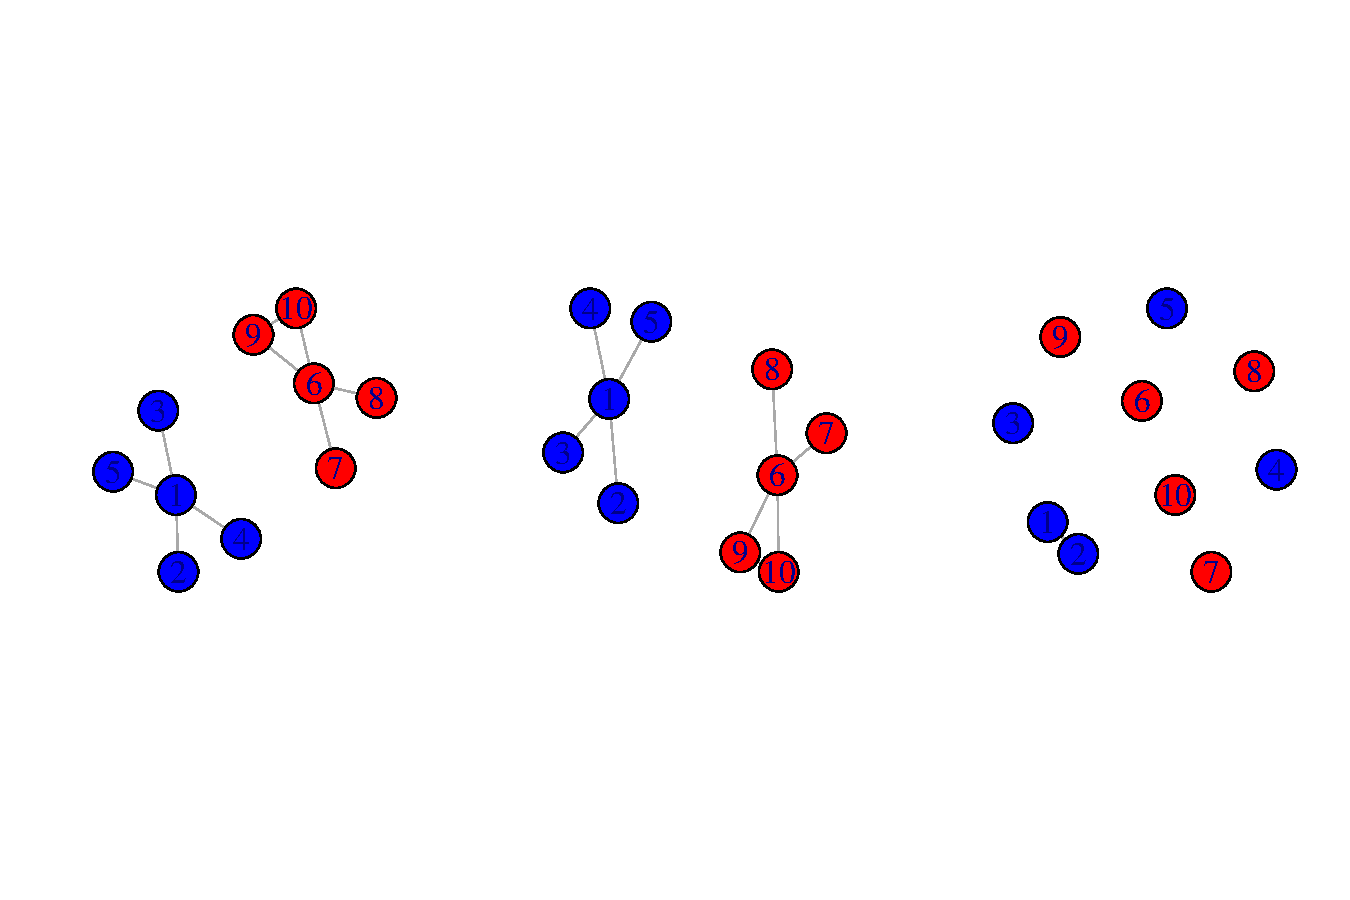
\includegraphics[width=.8\textwidth]{figures/r_inference_glasso_cor_res-1} 

\end{knitrout}
\end{frame}

\begin{frame}[fragile]
  \frametitle{A bit of code to run a simulation}

\begin{knitrout}\scriptsize
\definecolor{shadecolor}{rgb}{0.969, 0.969, 0.969}\color{fgcolor}\begin{kframe}
\begin{alltt}
\hlkwd{suppressMessages}\hlstd{(}\hlkwd{require}\hlstd{(reshape2))}
\hlstd{one.simu} \hlkwb{<-} \hlkwa{function}\hlstd{(}\hlkwc{i}\hlstd{) \{}
  \hlstd{lbd.c} \hlkwb{<-} \hlkwd{seq}\hlstd{(}\hlnum{1}\hlstd{,} \hlnum{0}\hlstd{,} \hlopt{-}\hlnum{10}\hlopt{^-}\hlnum{2}\hlstd{);}
  \hlstd{d} \hlkwb{<-} \hlnum{25}\hlstd{; seq.n} \hlkwb{<-} \hlkwd{c}\hlstd{(}\hlnum{10}\hlstd{,} \hlnum{15}\hlstd{,} \hlnum{30}\hlstd{,} \hlnum{50}\hlstd{,} \hlnum{100}\hlstd{,} \hlnum{150}\hlstd{,} \hlnum{300}\hlstd{,} \hlnum{500}\hlstd{)}
  \hlstd{out} \hlkwb{<-} \hlkwd{data.frame}\hlstd{(}\hlkwd{t}\hlstd{(}\hlkwd{sapply}\hlstd{(seq.n,} \hlkwa{function}\hlstd{(}\hlkwc{n}\hlstd{) \{}
   \hlstd{exp} \hlkwb{<-} \hlkwd{huge.generator}\hlstd{(n, d,} \hlkwc{graph}\hlstd{=}\hlstr{"cluster"}\hlstd{,}
                         \hlkwc{g}\hlstd{=}\hlnum{3}\hlstd{,} \hlkwc{prob}\hlstd{=}\hlnum{1}\hlstd{,} \hlkwc{verbose}\hlstd{=F)}
   \hlstd{gl} \hlkwb{<-} \hlkwd{huge}\hlstd{(exp}\hlopt{$}\hlstd{data,} \hlkwc{method}\hlstd{=}\hlstr{"glasso"}\hlstd{,} \hlkwc{nlambda}\hlstd{=}\hlnum{50}\hlstd{,} \hlkwc{verbose}\hlstd{=F)}
   \hlstd{mb} \hlkwb{<-} \hlkwd{huge}\hlstd{(exp}\hlopt{$}\hlstd{data,} \hlkwc{method}\hlstd{=}\hlstr{"mb"}\hlstd{,} \hlkwc{nlambda}\hlstd{=}\hlnum{50}\hlstd{,} \hlkwc{verbose}\hlstd{=F)}
   \hlstd{cthr} \hlkwb{<-} \hlkwd{huge}\hlstd{(exp}\hlopt{$}\hlstd{data,} \hlkwc{method}\hlstd{=}\hlstr{"ct"}\hlstd{,} \hlkwc{lambda}\hlstd{=lbd.c,} \hlkwc{verbose}\hlstd{=F)}
   \hlstd{res.cthr} \hlkwb{<-} \hlkwd{perf.auc}\hlstd{(}\hlkwd{perf.roc}\hlstd{(cthr}\hlopt{$}\hlstd{path, exp}\hlopt{$}\hlstd{theta))}
   \hlstd{res.gl} \hlkwb{<-} \hlkwd{perf.auc}\hlstd{(}\hlkwd{perf.roc}\hlstd{(gl}\hlopt{$}\hlstd{path, exp}\hlopt{$}\hlstd{theta))}
   \hlstd{res.mb} \hlkwb{<-} \hlkwd{perf.auc}\hlstd{(}\hlkwd{perf.roc}\hlstd{(mb}\hlopt{$}\hlstd{path, exp}\hlopt{$}\hlstd{theta))}
   \hlkwd{return}\hlstd{(}\hlkwd{setNames}\hlstd{(}\hlkwd{c}\hlstd{(res.gl,res.cthr,res.mb,n,i),}
   \hlkwd{c}\hlstd{(}\hlstr{"glasso"}\hlstd{,}\hlstr{"correlation"}\hlstd{,}\hlstr{"mb"}\hlstd{,} \hlstr{"sample size"}\hlstd{,} \hlstr{"simu"}\hlstd{)))}
  \hlstd{\})))}
\hlkwd{return}\hlstd{(}\hlkwd{melt}\hlstd{(out,} \hlkwc{measure.vars} \hlstd{=} \hlnum{1}\hlopt{:}\hlnum{3}\hlstd{,} \hlkwc{value.name} \hlstd{=} \hlstr{"score"}\hlstd{))\}}
\end{alltt}
\end{kframe}
\end{knitrout}

\end{frame}


\begin{frame}[fragile]
  \frametitle{Run}

\begin{knitrout}\scriptsize
\definecolor{shadecolor}{rgb}{0.969, 0.969, 0.969}\color{fgcolor}\begin{kframe}
\begin{alltt}
\hlkwd{suppressMessages}\hlstd{(}\hlkwd{library}\hlstd{(parallel))}
\hlstd{res} \hlkwb{<-} \hlkwd{do.call}\hlstd{(rbind,} \hlkwd{mclapply}\hlstd{(}\hlnum{1}\hlopt{:}\hlnum{40}\hlstd{, one.simu,} \hlkwc{mc.cores}\hlstd{=}\hlnum{4}\hlstd{))}
\end{alltt}
\end{kframe}
\end{knitrout}

\end{frame}

\begin{frame}[fragile]
  \frametitle{Simulation results (cluster - clique)}

\begin{knitrout}\scriptsize
\definecolor{shadecolor}{rgb}{0.969, 0.969, 0.969}\color{fgcolor}
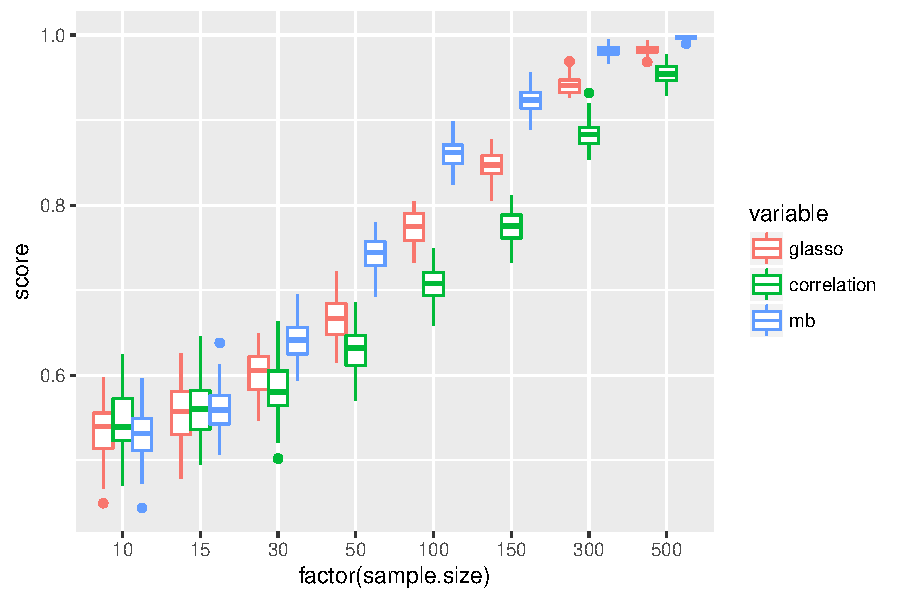
\includegraphics[width=.8\textwidth]{figures/r_plot_simu_cluster-1} 

\end{knitrout}




\end{frame}


\begin{frame}[fragile]
  \frametitle{Simulation results (cluster, connection probability of 0.5)}

\begin{knitrout}\scriptsize
\definecolor{shadecolor}{rgb}{0.969, 0.969, 0.969}\color{fgcolor}
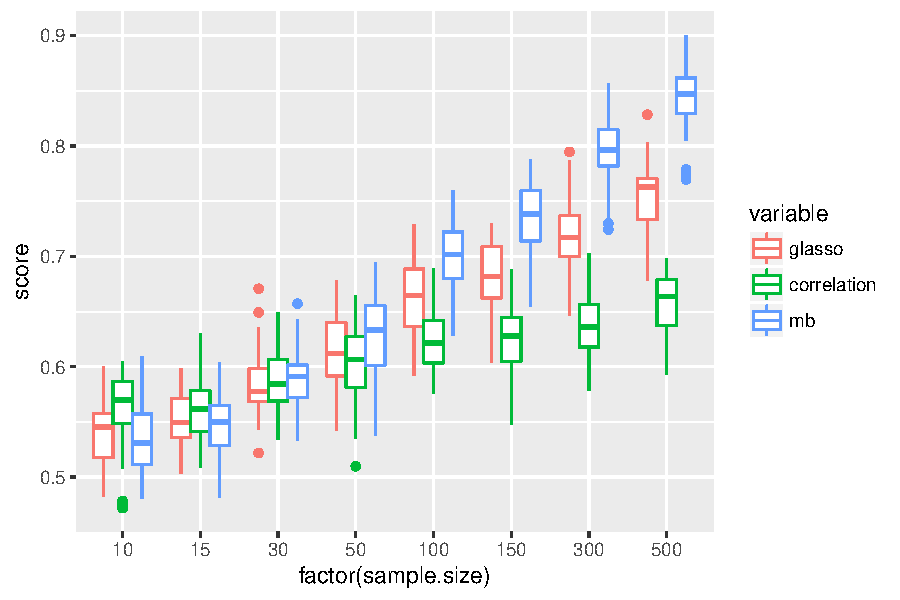
\includegraphics[width=.8\textwidth]{figures/r_plot_simu_cluster2-1} 

\end{knitrout}



\end{frame}

\begin{frame}[fragile]
  \frametitle{Simulation results (random, connection probability of 0.3)}

\begin{knitrout}\scriptsize
\definecolor{shadecolor}{rgb}{0.969, 0.969, 0.969}\color{fgcolor}
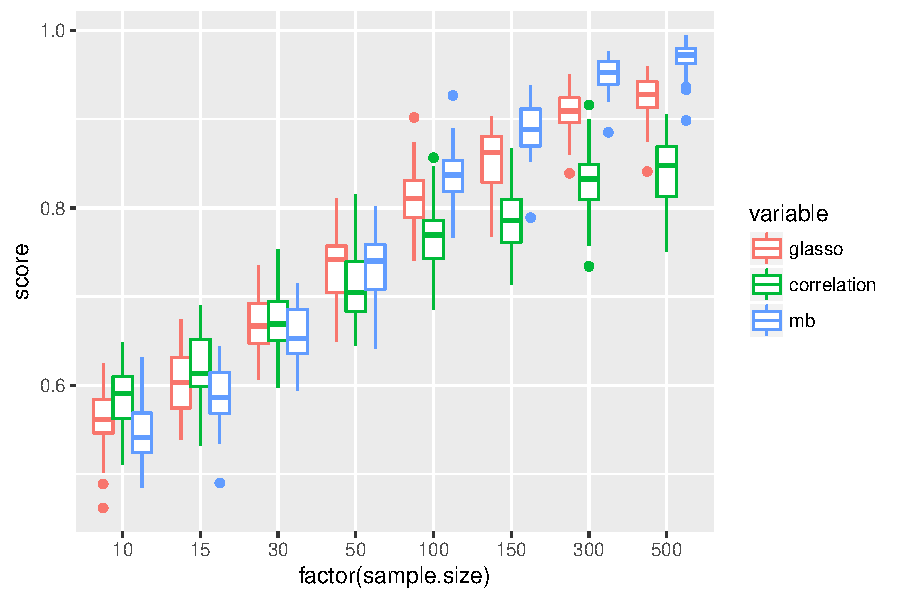
\includegraphics[width=.8\textwidth]{figures/r_plot_simu_random-1} 

\end{knitrout}

\end{frame}

\begin{frame}[fragile]
  \frametitle{Breast cancer: transcriptomics for ER+ and ER- tumors}

We look at a large public datasets from Guedj et al. 2011 with two main subgroups
  \begin{itemize}
  \item Estrogen receptor positive
  \item Estrogen receptor negative
  \end{itemize}

\begin{knitrout}\scriptsize
\definecolor{shadecolor}{rgb}{0.969, 0.969, 0.969}\color{fgcolor}\begin{kframe}
\begin{alltt}
\hlkwd{load} \hlstd{(}\hlstr{"huge/breast_cancer_guedj11.RData"}\hlstd{)}
\hlkwd{load} \hlstd{(}\hlstr{"huge/gen_name.RData"}\hlstd{)}
\hlstd{gene.name} \hlkwb{<-} \hlkwd{unlist}\hlstd{(gene.name)}
\hlstd{data.raw} \hlkwb{<-} \hlstd{expr}
\hlkwd{table}\hlstd{(class.ER)}
\end{alltt}
\begin{verbatim}
## class.ER
## ERm ERp 
## 162 375
\end{verbatim}
\end{kframe}
\end{knitrout}

\end{frame}

\begin{frame}[fragile]
  \frametitle{Filtering Unknown genes}

\begin{knitrout}\scriptsize
\definecolor{shadecolor}{rgb}{0.969, 0.969, 0.969}\color{fgcolor}\begin{kframe}
\begin{alltt}
\hlstd{toDiscard} \hlkwb{<-} \hlkwd{which}\hlstd{(gene.name} \hlopt{==} \hlstr{"Not.Known"}\hlstd{)}
\hlstd{gene.name} \hlkwb{<-} \hlstd{gene.name[}\hlopt{-}\hlstd{toDiscard]}
\hlstd{data.raw} \hlkwb{<-} \hlstd{data.raw[}\hlopt{-}\hlstd{toDiscard, ]}
\end{alltt}
\end{kframe}
\end{knitrout}

We get

\begin{knitrout}\scriptsize
\definecolor{shadecolor}{rgb}{0.969, 0.969, 0.969}\color{fgcolor}\begin{kframe}
\begin{alltt}
\hlkwd{dim}\hlstd{(data.raw)}
\end{alltt}
\begin{verbatim}
## [1] 41248   537
\end{verbatim}
\end{kframe}
\end{knitrout}

\end{frame}


\begin{frame}[fragile]
  \frametitle{Differential analysis}
  
Do we detect some gene expression differences ?

\begin{knitrout}\scriptsize
\definecolor{shadecolor}{rgb}{0.969, 0.969, 0.969}\color{fgcolor}\begin{kframe}
\begin{alltt}
\hlkwd{load} \hlstd{(}\hlstr{"huge/breast_cancer_guedj11.RData"}\hlstd{)}
\hlkwd{suppressMessages}\hlstd{(}\hlkwd{library}\hlstd{(limma))}
\hlstd{design} \hlkwb{<-} \hlkwd{cbind}\hlstd{(}\hlkwc{Moy}\hlstd{=}\hlnum{1}\hlstd{,} \hlkwc{Erp}\hlstd{=(class.ER} \hlopt{==} \hlstr{"ERp"}\hlstd{)}\hlopt{+}\hlnum{0}\hlstd{)}
\hlstd{fit} \hlkwb{<-} \hlkwd{lmFit}\hlstd{(data.raw,} \hlkwc{design}\hlstd{=design)}
\hlstd{fit} \hlkwb{<-} \hlkwd{eBayes}\hlstd{(fit)}
\hlstd{res} \hlkwb{<-} \hlkwd{topTable}\hlstd{(fit,} \hlkwc{coef}\hlstd{=}\hlstr{"Erp"}\hlstd{,} \hlkwc{number}\hlstd{=}\hlnum{10}\hlopt{^}\hlnum{5}\hlstd{,}
                \hlkwc{genelist}\hlstd{=fit}\hlopt{$}\hlstd{genes,} \hlkwc{adjust.method}\hlstd{=}\hlstr{"BH"}\hlstd{,}
              \hlkwc{sort.by}\hlstd{=}\hlstr{"none"}\hlstd{,} \hlkwc{resort.by}\hlstd{=}\hlkwa{NULL}\hlstd{,}
              \hlkwc{p.value}\hlstd{=}\hlnum{1}\hlstd{,} \hlkwc{lfc}\hlstd{=}\hlnum{0}\hlstd{,} \hlkwc{confint}\hlstd{=}\hlnum{FALSE}\hlstd{)}
\end{alltt}
\end{kframe}
\end{knitrout}

\end{frame}



\begin{frame}[fragile]
  \frametitle{Many genes are differentially expressed}

\begin{itemize}
\item The histogram of p-values looks good
\item This is a well known fact (ER+ and ER- are very different)
\end{itemize}

\begin{knitrout}\scriptsize
\definecolor{shadecolor}{rgb}{0.969, 0.969, 0.969}\color{fgcolor}\begin{kframe}
\begin{alltt}
\hlkwd{sum}\hlstd{(res}\hlopt{$}\hlstd{adj.P.Val} \hlopt{<} \hlnum{10}\hlopt{^-}\hlnum{5}\hlstd{)}
\end{alltt}
\begin{verbatim}
## [1] 5907
\end{verbatim}
\begin{alltt}
\hlkwd{hist}\hlstd{(res}\hlopt{$}\hlstd{P.Value,} \hlkwc{breaks}\hlstd{=}\hlnum{30}\hlstd{,} \hlkwc{col}\hlstd{=}\hlstr{"grey"}\hlstd{,}
     \hlkwc{main}\hlstd{=}\hlstr{"P-values ER- vs ER+"}\hlstd{)}
\end{alltt}
\end{kframe}
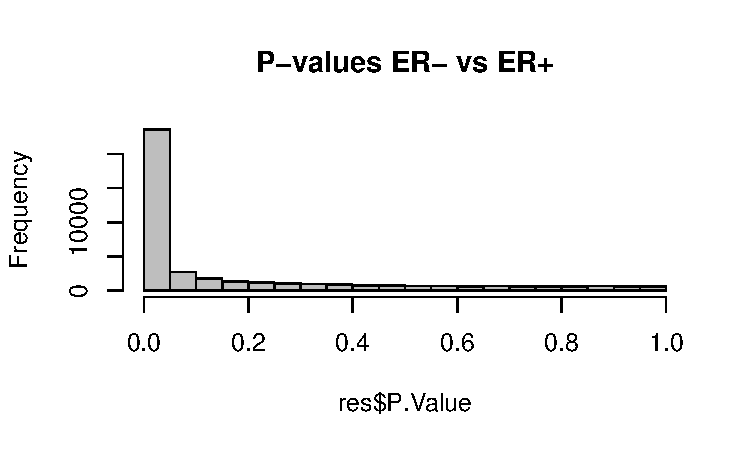
\includegraphics[width=.8\textwidth]{figures/r_many_genes-1} 

\end{knitrout}

\end{frame}

\begin{frame}[fragile]
  \frametitle{What to do with this list of genes?}

ESR1 has the most significant p-values

\begin{knitrout}\scriptsize
\definecolor{shadecolor}{rgb}{0.969, 0.969, 0.969}\color{fgcolor}\begin{kframe}
\begin{alltt}
\hlstd{gene.name[}\hlkwd{order}\hlstd{(res}\hlopt{$}\hlstd{adj.P.Val)[}\hlnum{1}\hlstd{]]}
\end{alltt}
\begin{verbatim}
## 205225_at 
##    "ESR1"
\end{verbatim}
\end{kframe}
\end{knitrout}

\begin{block}{Network analysis}
\begin{itemize}
\item Could we find partners of ESR1 that are specific to ER+?
\item We cannot infer a network on  41000 genes (Verzelen 2011)
\begin{itemize}
\item[\rsa] \emphase{Most differentially expressed} genes
\item[\rsa] Most varying genes
\item[\rsa] Look at a specific pathway \dots
\end{itemize}
\end{itemize}
\end{block}

\end{frame}

\begin{frame}[fragile]
  \frametitle{Selecting some probes}

Take the 20 most differentially expressed plus some random



\begin{knitrout}\scriptsize
\definecolor{shadecolor}{rgb}{0.969, 0.969, 0.969}\color{fgcolor}\begin{kframe}


{\ttfamily\noindent\bfseries\color{errorcolor}{\#\# Error in graph\_from\_adjacency\_matrix(net\_Mspec\_): could not find function "{}graph\_from\_adjacency\_matrix"{}}}

{\ttfamily\noindent\bfseries\color{errorcolor}{\#\# Error in graph\_from\_adjacency\_matrix(net\_Pspec\_): could not find function "{}graph\_from\_adjacency\_matrix"{}}}\end{kframe}
\end{knitrout}

\begin{knitrout}\scriptsize
\definecolor{shadecolor}{rgb}{0.969, 0.969, 0.969}\color{fgcolor}
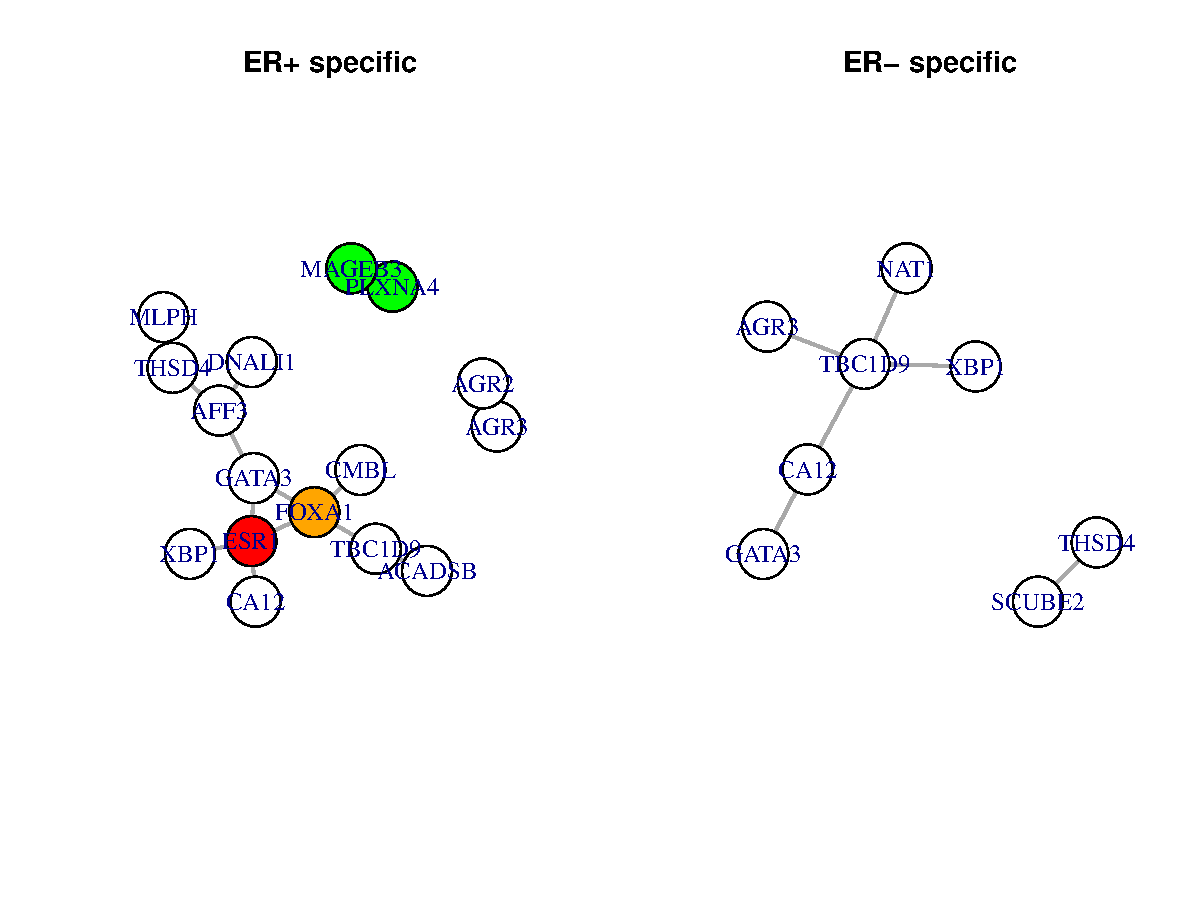
\includegraphics[width=.8\textwidth]{figures/r_ploting_network_random-1} 

\end{knitrout}


\end{frame}

\begin{frame}[fragile]
  \frametitle{FOXA1, ESR1, GATA3 a well known interaction}

\begin{enumerate}
\item FOXA1 is a key determinant of estrogen receptor function and endocrine response. Antoni Hurtado et al. 2011 (Nat. Genet.):

    \rsa "FOXA1 is a key determinant that can influence differential interactions between ER and chromatin"

\item GATA3 acts upstream of FOXA1 in mediating ESR1 binding by shaping enhancer accessibility. Theodorou et al. 2013 (Genome Res.)

\item Estrogen receptor regulation of carbonic anhydrase XII through a distal enhancer in breast cancer.
Barnett DH et al 2008 (Cancer Res.)
    
    \rsa "we show that CA12 is robustly regulated by estrogen via ER alpha in breast cancer cells"
\end{enumerate}

\end{frame}


\part<presentation>{Extensions}
\begin{frame}
  \partpage
  \tableofcontents[hideallsubsections]
\end{frame}

\begin{frame}
  \frametitle{Extensions motivated by biological data}

  \begin{block}{\alert{Strengthen the inference } by}
    \vspace{-.25cm}

    \begin{itemize}
    \item accounting for biological features

      \begin{enumerate}
      \item \alert{structure} of the network (organization of biological mechanisms)
      \item sample \alert{heterogeneity} (structure of the population)
      \item horizontal \alert{integration} (use multiple data and platforms)
      \item Deal with \alert{covariates}
      \end{enumerate}

    \item accounting for data features

      \begin{enumerate}
      \item What if some \alert{important actor is missing}?
      \item Extend to \alert{non strictly normal} distribution
      \item Deal with a \alert{large number} of actors
      \end{enumerate}
    \end{itemize}

  $\rightsquigarrow$ How? Essentially by crafting the regularization according to our prior knowledge

  \end{block}

\end{frame}

\pgfdeclareimage[height=0.5\textheight]{optim}{figures/fig_optim2}

\begin{frame}
  \frametitle{General strategy}
  \framesubtitle{Revisit ``traditional'' statistical methods under the light of optimization}
  
  \begin{overlayarea}{\textwidth}{\textheight}
    
    \begin{enumerate}
      \item statistical problem $\leftrightarrow$ optimization problem
          \begin{equation*}
          \minimize_{\btheta}     L(\btheta;\textbf{data})    \quad
          \text{s.t.} \quad \Omega(\btheta) \leq c.
          \end{equation*}

      \item  modification  of  the original  problem/regularization
          \begin{columns}
            \begin{column}{0.5\textwidth}
              \begin{tikzpicture}
                \node (surf) at (0,0) {\pgfuseimage{optim}}
                node at (surf.west) [rotate=90,yshift=-5mm,xshift=0mm] {\footnotesize$L(\theta_1,\theta_2;\textbf{data})$}
                node at (surf.south west) [xshift=10mm,yshift=5mm]{\footnotesize$\theta_2$}
                node at (surf.south east) [xshift=-20mm,yshift=1mm]{\footnotesize$\theta_1$};
              \end{tikzpicture}
            \end{column}
            \begin{column}{0.5\textwidth}
              \begin{footnotesize}
                modify $\Omega$ and/or $L$ to
                \begin{itemize}
                \item \footnotesize control the computational cost
                \item \footnotesize control the model complexity
                \item \footnotesize account for  prior knowledge
                \end{itemize}
                looking for
                \begin{itemize}
                \item[$\rightsquigarrow$] \footnotesize $\uparrow$ performance and interpretability
                \item[$\rightsquigarrow$] \footnotesize trade-off between speed and accuracy
                \end{itemize}
              \end{footnotesize}
            \end{column}
          \end{columns}
      \end{enumerate}
  \end{overlayarea}

\end{frame}

%% account for underlying structure of the network
\section{Accounting for latent organisation of the network}

\begin{frame}
  \frametitle{Handling with the data structure and scarcity}
  \framesubtitle{By introducing some prior}

  \begin{block}{Priors should be biologically grounded}
    \begin{enumerate}
    \item no too many genes effectively interact: \alert{sparsity},
    \item networks are organized: \alert{latent clustering}.
    \end{enumerate}
  \end{block}

  \vfill

  \begin{center}
    \begin{overlayarea}{\textheight}{\textwidth}
      \begin{scriptsize}
        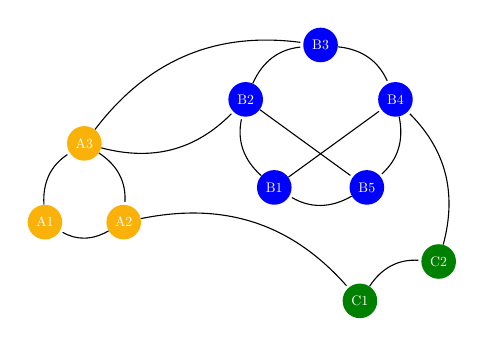
\begin{tikzpicture}
          %% UN GRAPH
          \tikzstyle{every edge}=[-,>=stealth',shorten >=1pt,auto,thin,draw]
          \tikzstyle{every state}=[draw=none,text=white,scale=0.5, transform shape]

          \tikzstyle{every node}=[fill=yellow!40!orange]
          % premier cluster
          \node[state] (A1) at (1,0.5) {A1};
          \node[state] (A2) at (2,0.5) {A2};
          \node[state] (A3) at (1.5,1.5) {A3};

          \path (A2) edge [bend left,] (A1)
          (A1) edge [bend left] (A3)
          (A3) edge [bend left] (A2);

          \tikzstyle{every node}=[fill=blue!80!black]
          \foreach \angle/\text in {234/B1, 162/B2, 90/B3, 18/B4, -54/B5} {
            \node[fill=blue,state,xshift=9cm,yshift=3.5cm]     (\text)    at
            (\angle:1cm) {\text};
          }
          \path (B2) edge (B5)
          (B1) edge (B4);
          \foreach \from/\to in {1/2,2/3,3/4,4/5,5/1}{
            \path (B\from) edge [bend left] (B\to);
          }

          \tikzstyle{every node}=[fill=green!50!black]
          % troisime cluster
          \node[state] (C1) at (5,-.5) {C1};
          \node[state] (C2) at (6,0) {C2};

          \path (C1) edge [bend left] (C2);

          % inter cluster
          \path (A3) edge [bend right] (B2)
          (A3) edge [bend left] (B3)
          (C2) edge [bend right] (B4)
          (A2) edge [bend left] (C1);
        \end{tikzpicture}
      \end{scriptsize}
    \end{overlayarea}
  \end{center}

 \end{frame}

\begin{frame}
  \frametitle{Structured regularization}

  \begin{block}{SIMoNe: Statistical Inference for MOdular NEtworks}
    \begin{equation*}
      \argmax_{\bTheta,\mathbf{Z}}
      \ell(\bTheta;\mathbf{Y}) -
      \lambda \
      \|\mathbf{P}_{\mathbf{Z}}\star \bTheta\|_{\ell_1},
    \end{equation*}
    where $\mathbf{P}_{\mathbf{Z}}$  is a matrix of  weights depending
    on  a \alert{underlying}  latent structure  $\mathbf{Z}$ (depicted
    through a stochastic block model).

    \medskip

    $\rightsquigarrow$   \alert{Cluster-driven   inference}  via   an
    \textsc{EM}-like strategy.
  \end{block}

  \vspace{.5cm}

  \begin{thebibliography}{99}
    \begin{scriptsize}
    \bibitem[CJC]{CJC} Ambroise, Chiquet, Matias. Inferring sparse GGM with
      latent structure, \textcolor{black}{EJS}, 2009.
    \bibitem[UCI]{UCI} Marlin, Schmidt,  Murphy: similar Bayesian work
      \textcolor{black}{UCI} 2010.
    \bibitem[W14]{W14}  Wong et  al.,  close update:  \textit{Adaptive
        Graphical Lasso}, 2014.
    \end{scriptsize}
  \end{thebibliography}

   \defbeamertemplate{bibliography item}{package}{\pgfuseimage{computer}}
   \setbeamertemplate{bibliography item}[package]

  \begin{thebibliography}{99}
    \begin{scriptsize}
    \bibitem[simone]{simone} Chiquet et al., SIMoNe
      \texttt{R}-package \textit{(needs updates\dots)}, Note
      Bioinformatics, 2009.
    \end{scriptsize}
  \end{thebibliography}
  
\end{frame}

% \begin{frame}
%   \frametitle{Structured regularization}
%   \framesubtitle{``Bayesian'' interpretation of $\ell_1$ regularization}

%   \begin{block}{Laplacian prior  on $\bTheta$ depends on  the clustering
%       $\mathbf{Z}$}
%     \begin{equation*}
%       \mathbb{P}(\bTheta|\mathbf{Z}) \propto \prod_{i,j} 
%       \exp\left\{-\lambda \cdot \mathbf{P}^{\mathbf{Z}}_{ij} \cdot |\bTheta_{ij}|\right\}.
%     \end{equation*}
%   \end{block}

%   \begin{block}{$\mathbf{P}_{\mathbf{Z}}$ summarizes prior information
%       on the position of edges}
%     \vspace{-2ex}
%     \centering
%     \includegraphics[width=.45\textwidth]{figures/laplacian_prior.pdf}
%   \end{block}
  
% \end{frame}

\begin{frame}
  \frametitle{How to come up with a latent clustering?}
  
  \begin{block}{Biological expertise}
    \begin{itemize}
    \item Build $\mathbf{Z}$ from prior biological information 
      \begin{itemize}
      \item transcription factors vs. regulatees,
      \item number of potential binding sites,
      \item KEGG pathways, \dots
      \end{itemize}
    \item Build the weight matrix from $\mathbf{Z}$.
    \end{itemize}
  \end{block}
  
  \vfill
  
  \begin{block}{Inference: Erdös-Rényi  \textbf{Mix}ture for
      \textbf{Net}works \\ \small{(Daudin et al., 2008; Latouche et al., 2011)}} 
    \begin{itemize}
    \item Equivalent to the Stochastic Bloc Model (SBM);
    \item    Spread the  nodes into $\mathcal{Q}$ classes;
    \item Connexion probabilities depend upon node classes:
      \begin{equation*}
        \mathbb{P} (i \leftrightarrow j|i \in \mathsf{ class}\ q, j \in
        \mathsf{ class }\ \ell) = \pi_{q \ell}.
      \end{equation*}
    \item Build $P_{\mathbf{Z}} \propto 1-\pi_{q\ell}$.
    \end{itemize}
   \end{block}
\end{frame}

\begin{frame}
  \frametitle{Illustration on breast Cancer}
  \framesubtitle{Prediction   of    the   outcome    of   preoperative
    chemotherapy}
  \begin{overlayarea}{\textwidth}{1.1\textheight}
    \begin{columns}[c]
      \begin{column}{.35\textwidth}
        
        \begin{thebibliography}{99}
          \begin{footnotesize}
          \bibitem{hess}  Hess \textit{et  al.}   \newblock Journal.  of
            Clinical Oncology, 2006.
          \end{footnotesize}
        \end{thebibliography}
        
        \begin{block}{Data set}
          \small 133 patients classified as
          \begin{enumerate}
          \item \small pathologic complete response,
          \item \small residual disease,
          \end{enumerate}
          according to a signature of 26 genes (small network).
        \end{block}
      \end{column}
      
      \begin{column}{.65\textwidth}
        \begin{figure}
          \centering
          \includegraphics<1>[width=\textwidth]{hess_noclust}
          \includegraphics<2>[width=\textwidth]{breast_thirtyedges}
          \small\caption{Pooling the data, \only<1>{Neighborhood Selection}\only<2>{SIMoNE with clustering}}
        \end{figure}
      \end{column}
    \end{columns}
  \end{overlayarea}
  
\end{frame}


%% account for sample heterogeneity
\section{Accouting for sample heterogeneity}

\begin{frame}
  \frametitle{Handling scarcity and heterogeneity of data}

  \label{multi:scheme}
    
    \only<1>{Merge several experimental conditions}
    \only<2>{Inferring each graph \alert{independently} does not help}
    \only<3>{By \alert{pooling}  all the available data  (like we just
      have with Hess' data set)}
    \only<4->{By \alert{breaking} the separability}
  
  \vfill
  
  \begin{overlayarea}{\textwidth}{\textheight}
    
  \begin{tikzpicture}
    
    %% DATA 1
    \node at (-4.5,-0) {condition 1};
    \node[opacity=.75] (puce1)  at (-4.5,-1) {\pgfuseimage{ngs}};
    \node[opacity=.9]  (puce1b) at (-4.25,-1.25) {\pgfuseimage{ngs}};
    \node[opacity=.95] (puce1c) at (-4,-1.5) {\pgfuseimage{ngs}};
    
    %% DATA 2
    \node at (0,-0) {condition 2};
    \node[opacity=.75] (puce2)  at (0,-1) {\pgfuseimage{ngs}};
    \node[opacity=.9]  (puce2b) at (.25,-1.25) {\pgfuseimage{ngs}};
    \node[opacity=.95] (puce2c) at (.5,-1.5) {\pgfuseimage{ngs}};
    
    %% DATA 3
    \node at (4.5,-0) {condition 3};
    \node[opacity=.75] (puce3)  at (4.5,-1) {\pgfuseimage{ngs}};
    \node[opacity=.9]  (puce3b) at (4.75,-1.25) {\pgfuseimage{ngs}};
    \node[opacity=.95] (puce3c) at (5,-1.5) {\pgfuseimage{ngs}};
         
    %% independent inference
    \only<2,4-5>{
      \node (data1) at (-4,-2.75) {%
        \sf\scriptsize $(Y_1^{(1)},\dots,Y_{n_1}^{(1)})$
      };
      \node (data2) at (0.5,-2.75) {%
        \sf \scriptsize $(Y_1^{(2)},\dots,Y_{n_2}^{(2)})$
      };
      \node (data3) at (5,-2.75) {%
        \sf \scriptsize $(Y_1^{(3)},\dots,Y_{n_3}^{(3)})$
      };

      \path[->] (puce1c) edge (data1);
      \path[->] (puce2c) edge (data2);
      \path[->] (puce3c) edge (data3);

      \node[fill=red, text=white,single arrow, shape border rotate =270] 
      (inference1) at (-4,-3.25) {\sf \scriptsize inference}; 
      
      \node[fill=red, text=white,single arrow, shape border rotate =270] 
      (inference2) at (0.5,-3.25) {\sf \scriptsize inference}; 
      
      \node[fill=red, text=white,single arrow, shape border rotate =270] 
      (inference3) at (5,-3.25) {\sf \scriptsize inference}; 

   }
    \only<2>{
      %% GRAPH SETTINGS
      \tikzstyle{every edge}=[-,>=stealth',shorten >=1pt,auto,thin,draw]
      \tikzstyle{every node}=[fill=orange!70!white]
      \tikzstyle{every state}=[draw=none,text=white,scale=0.25, transform shape] 
      
      %% graph 1
      \node[state] (A1) at (-5.5,-6.0) {};
      \node[state] (A2) at (-5,-5.0) {};
      \node[state] (A3) at (-4.5,-6.0) {};
      \foreach \name/\angle/\text in {B1/234/G3, B2/162/G4, B4/18/G6, B3/90/G5, B5/-54/G7} {
        \node[state,xshift=-14cm,yshift=-21cm]     (\name)    at
        (\angle:.5cm) {}; }
 
      \path (A2) edge [bend left] (B3)
      (A2) edge [bend right] (A1) 
      (A3) edge [bend right] (A2)
      (A3) edge (B2) 
      (B1) edge [bend left] (B3)
      (A3) edge [bend right] (B3);
      
      \path (B1) edge [bend right] (A1);
      \foreach \from/\to in {1/2,2/3}{
        \path (B\from) edge [bend left] (B\to);
      }
      
      %% graph 2
      \node[state] (A1) at (-1,-6.0) {};
      \node[state] (A2) at (-0.5,-5.0) {};
      \node[state] (A3) at (0,-6.0) {};
      \foreach \name/\angle/\text in {B1/234/G3, B2/162/G4, B4/18/G6, B3/90/G5, B5/-54/G7} {
        \node[state,xshift=4cm,yshift=-21cm]     (\name)    at
        (\angle:.5cm) {}; }
    
      \path % (A1) edge [bend right] (B5) 
      (A2) edge [bend left] (B3)
      (A2) edge [bend right] (A1) 
      (A1) edge  (A3);
      
      \path (B1) edge [bend right] (A1);
      \foreach \from/\to in {1/3,3/5,5/1}{
        \path (B\from) edge [bend left] (B\to);
      }
      
      %% graph 3
      \node[state] (A1) at (3,-6.0) {};
      \node[state] (A2) at (3.5,-5.0) {};
      \node[state] (A3) at (4,-6.0) {};
      \foreach \name/\angle/\text in {B1/234/G3, B2/162/G4, B4/18/G6, B3/90/G5, B5/-54/G7} {
        \node[state,xshift=20cm,yshift=-21cm]     (\name)    at
        (\angle:.5cm) {}; }
      
      \path (A3) edge [bend right] (A2)
      (A3) edge (B2);
      
      \path (B1) edge (B4);
      \foreach \from/\to in {1/2,4/5,5/1,2/4}{
        \path (B\from) edge [bend left] (B\to);
      }
    }

    %% pooled inference
    \only<3>{
      \node (pooled) at (0.5,-2.75) {%
        \sf \scriptsize $(Y_1,\dots,Y_{n})$, $n=n_1+n_2+n_3$.
      };

      \path[->] (puce1c) edge (pooled);
      \path[->] (puce3c) edge (pooled);
      \path[->] (puce2c) edge (pooled);

      %% GRAPH SETTINGS
      \tikzstyle{every edge}=[-,>=stealth',shorten >=1pt,auto,thin,draw]
      \tikzstyle{every node}=[fill=orange!70!white]
      \tikzstyle{every state}=[draw=none,text=white,scale=0.25, transform shape] 
      
      \node[state] (A1) at (-1,-6.0) {};
      \node[state] (A2) at (-0.5,-5.0) {};
      \node[state] (A3) at (0,-6.0) {};
      \foreach \name/\angle/\text in {B1/234/G3, B2/162/G4, B4/18/G6, B3/90/G5, B5/-54/G7} {
        \node[state,xshift=4cm,yshift=-21cm]     (\name)    at
        (\angle:.5cm) {}; }
    
      \path % (A1) edge [bend right] (B5) 
      (A2) edge [bend left] (B3)
      (A2) edge [bend right] (A1)
      (A1) edge  (A3)
      (A3) edge [bend right] (A2)
      (A3) edge (B2) 
      (A3) edge [bend right] (B3);
      
      \path (B1) edge [bend right] (A1);
      \foreach \from/\to in {1/3,3/5,5/1,1/2,4/5,2/4}{
        \path (B\from) edge [bend left] (B\to);
      }
            
      \node[fill=red, text=white,single arrow, shape border rotate =270] 
      (inference) at (0.5,-3.25) {\sf \scriptsize inference}; 
    }

    %% multitask inference
    \only<4-5>{

      \path[->] (data1.east) edge [color=red] (inference2.west);
      \path[->] (data1.east) edge [color=red, bend right=5,in=175] (inference3.west);
      \path[->] (data2.west) edge [color=red] (inference1.east);
      \path[->] (data2.east) edge [color=red] (inference3.west);
      \path[->] (data3.west) edge [color=red, bend left=5,in=185] (inference1.east);
      \path[->] (data3.west) edge [color=red] (inference2.east);
    }
    \only<4>{

      %% GRAPH SETTINGS
      \tikzstyle{every edge}=[-,>=stealth',shorten >=1pt,auto,thin,draw]
      \tikzstyle{every node}=[fill=orange!70!white]
      \tikzstyle{every state}=[draw=none,text=white,scale=0.25, transform shape] 
      
      %% graph 1
      \node[state] (A1) at (-5.5,-6.0) {};
      \node[state] (A2) at (-5,-5.0) {};
      \node[state] (A3) at (-4.5,-6.0) {};
      \foreach \name/\angle/\text in {B1/234/G3, B2/162/G4, B4/18/G6, B3/90/G5, B5/-54/G7} {
        \node[state,xshift=-14cm,yshift=-21cm]     (\name)    at
        (\angle:.5cm) {}; }
 
      \path (A2) edge [bend left] (B3)
      (A2) edge [bend right] (A1) 
      (A1) edge  (A3)
      (A3) edge [bend right] (A2)
      (A3) edge (B2) 
      (B1) edge [bend left] (B3);
      
      \path (B1) edge [bend right] (A1);
      \foreach \from/\to in {1/2,2/3,3/5}{
        \path (B\from) edge [bend left] (B\to);
      }
      
      %% graph 2
      \node[state] (A1) at (-1,-6.0) {};
      \node[state] (A2) at (-0.5,-5.0) {};
      \node[state] (A3) at (0,-6.0) {};
      \foreach \name/\angle/\text in {B1/234/G3, B2/162/G4, B4/18/G6, B3/90/G5, B5/-54/G7} {
        \node[state,xshift=4cm,yshift=-21cm]     (\name)    at
        (\angle:.5cm) {}; }
    
      \path % (A1) edge [bend right] (B5) 
      (A2) edge [bend left] (B3)
      (A2) edge [bend right] (A1)
      (A3) edge (B2)
      (A1) edge  (A3) ;
      
      \path (B1) edge [bend right] (A1);
      \foreach \from/\to in {1/2,2/3,1/3,3/5,5/1}{
        \path (B\from) edge [bend left] (B\to);
      }
      
      %% graph 3
      \node[state] (A1) at (3,-6.0) {};
      \node[state] (A2) at (3.5,-5.0) {};
      \node[state] (A3) at (4,-6.0) {};
      \foreach \name/\angle/\text in {B1/234/G3, B2/162/G4, B4/18/G6, B3/90/G5, B5/-54/G7} {
        \node[state,xshift=20cm,yshift=-21cm]     (\name)    at
        (\angle:.5cm) {}; }
      
      \path (A3) edge [bend right] (A2)
      (A2) edge [bend left] (B3)
      (A3) edge (B2)
      (A1) edge  (A3) ;
      
      \path (B1) edge [bend right] (A1);
      \foreach \from/\to in {1/2,2/3,3/5,5/1}{
        \path (B\from) edge [bend left] (B\to);
      }
      
      \node[fill=red, text=white,single arrow, shape border rotate =270] 
      (inference) at (-4,-3.25) {\sf \scriptsize inference}; 
      
      \node[fill=red, text=white,single arrow, shape border rotate =270] 
      (inference) at (0.5,-3.25) {\sf \scriptsize inference}; 
      
      \node[fill=red, text=white,single arrow, shape border rotate =270] 
      (inference) at (5,-3.25) {\sf \scriptsize inference};       
    }
  \end{tikzpicture}

  \begin{block}{Multiple inference of GGM}<5>
    \begin{equation*}
      \argmax_{\boldsymbol\Theta^{(c)}, c=1\dots,C} 
      \sum_{c=1}^C
      \ell( \boldsymbol\Theta^{(c)};
      \mathbf{S}^{(c)}) -
      \lambda \ \mathrm{pen}_{\ell_1}(\boldsymbol\Theta^{(c)}).
    \end{equation*}
  \end{block}

\end{overlayarea}

\end{frame}

\begin{frame}
  \frametitle{A multitask approach}
  \framesubtitle{Chiquet, Grandvalet, Ambroise, Statistics and Computing 2010/11}

  \begin{overlayarea}{\textwidth}{\textheight}
    
  \begin{block}{Break the separability}
    Joint the optimization problem by either modifying
    \begin{equation*}
      \argmax_{\boldsymbol\Theta^{(c)}, c=1\dots,C} 
      \sum_{c=1}^C
      \tilde{\ell}(                           \boldsymbol\Theta^{(c)};
      \only<2>{\alert{\tilde{\mathbf{S}}^{(c)}}}\only<1,3>{\tilde{\mathbf{S}}^{(c)}})
      - \lambda \ \alert<3>{\mathrm{pen}_{\ell_1}(\boldsymbol\Theta^{(c)})}.
    \end{equation*}
  \begin{enumerate}
  \item \alert<2>{the fitting term}
  \item \alert<3>{the regularization term}
  \end{enumerate}
  \end{block}
  
  \only<2>{
    \begin{block}{Intertwined-Lasso}
      \begin{itemize}
      \item       $\overline{\mathbf{S}}       =      \frac{1}{n}\sum_{t=1}^T
        n_t\mathbf{S}^{(t)}$ is the ``pooled-tasks'' covariance matrix.
      \item $\widetilde{\mathbf{S}}^{(t)} = \alpha \mathbf{S}^{(t)} +
        (1-\alpha)\overline{\mathbf{S}}$ is a mixture between specific and pooled
        covariance matrices.
      \end{itemize}    
    \end{block}
  }
  
  \only<3>{
    \begin{block}{Sparsity with grouping effect}
      \begin{itemize}
      \item Group-Lasso (Yuan and Lin 2006, Grandvalet and Canu, 1998),
      \item Cooperative-Lasso (Chiquet et al, AoAS, 2012),
      \end{itemize}
    \end{block}
  }
  \end{overlayarea}
  
\end{frame}

\begin{frame}
  \frametitle{Grouping effects induced}

  \centering
  \begin{small}
    \begin{tabular}{lc@{\hspace{.1cm}}cc}
      & Potential groups & \multicolumn{2}{c}{Group(s) induced by edges $(1,2)$} \\
      \rotatebox{90}{\hspace{1cm}Group-\textsc{Lasso}} & 
      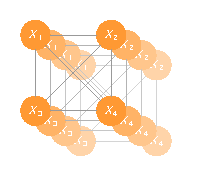
\includegraphics[width=.3\textwidth]{figures/grouping_grp_1} & 
      \multicolumn{2}{c}{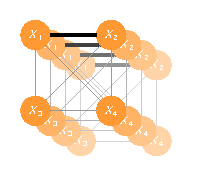
\includegraphics[width=.3\textwidth]{figures/grouping_grp_2}} \\
      \rotatebox{90}{\hspace{.35cm}Cooperative-\textsc{Lasso}} &
      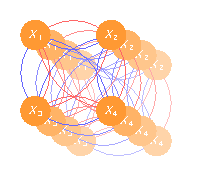
\includegraphics[width=.3\textwidth]{figures/grouping_coop_1} & 
      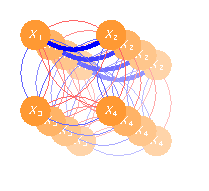
\includegraphics[width=.3\textwidth]{figures/grouping_coop_2} & 
      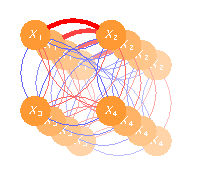
\includegraphics[width=.3\textwidth]{figures/grouping_coop_3} \\
    \end{tabular}
  \end{small}
\end{frame}


\begin{frame}
  \frametitle{Other grouping effects induced}

  \begin{beamerboxesrounded}[upper=sur:head,lower=sur:bloc,shadow=true]{Recent works}
    \begin{itemize}
    \item Use Fused-Lasso, sparse group-Lasso
    \item  Adapted several  time  to the  \alert{Graphical Lasso  framework}
      \begin{itemize}
        \item\scriptsize See, e.g. D. Witten's team works.
        \item\scriptsize The multitask/neighborhood selection's approach remains competitive.
        \end{itemize}
        \vspace{.5cm}
      \item Mohan et al., 2014
        \begin{itemize}
        \item\scriptsize   Networks  differences   are  only   due  to
          \alert{perturbations at the node level}.
        \item\scriptsize For instance, a hub is encouraged to be shared across tasks.
        \end{itemize}
      \end{itemize}
    \end{beamerboxesrounded}

\end{frame}

\begin{frame}
  \frametitle{Revisiting the Hess \textit{et al.} data set}
  
  \begin{figure}
    \centering
    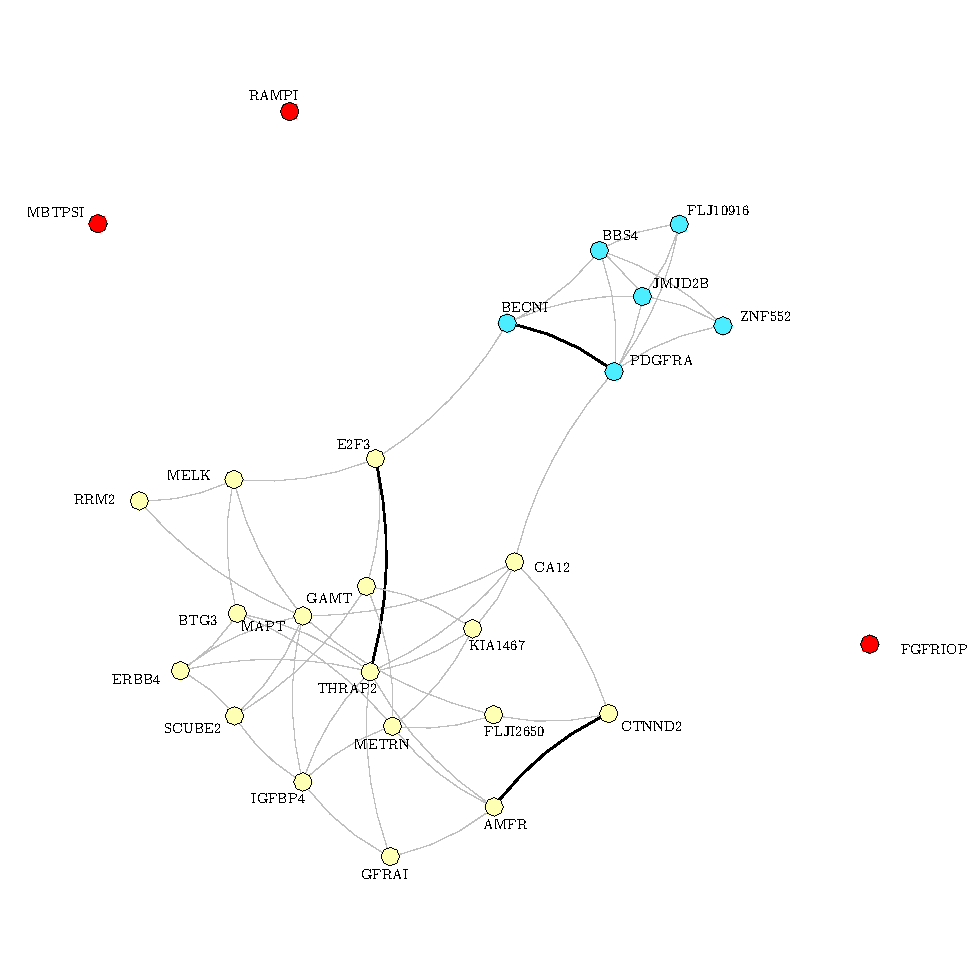
\includegraphics[width=.65\textwidth]{multi_breast}
    \caption{Cooperative-Lasso applied on the  two sets of patients
      (PCR/noPCR). Bold edges are different in the finally selection graph.} 
  \end{figure}

\end{frame}


%% account for multivariate data
\include{multiattribute}

%% Handling count data-> Poisson Log-normal

\section{Model for count data}



\begin{frame}[fragile]
  \frametitle{Motivations: oak powdery mildew pathobiome}

  \begin{block}{Metabarcoding data from [JFS16]}<1->
    \begin{itemize}
    \item $n = 116$ leaves, $p = 114$ species ($66$ bacteria, $47$ fungies + \textit{E. alphitoides})
\begin{knitrout}\scriptsize
\definecolor{shadecolor}{rgb}{0.969, 0.969, 0.969}\color{fgcolor}\begin{kframe}
\begin{alltt}
\hlstd{counts[}\hlnum{1}\hlopt{:}\hlnum{3}\hlstd{,} \hlkwd{c}\hlstd{(}\hlnum{1}\hlopt{:}\hlnum{4}\hlstd{,} \hlnum{48}\hlopt{:}\hlnum{51}\hlstd{)]}
\end{alltt}
\begin{verbatim}
##       f_1 f_2 f_3 f_4 E_alphitoides b_1045 b_109 b_1093
## A1.02  72   5 131   0             0      0     0      0
## A1.03 516  14 362   0             0      0     0      0
## A1.04 305  24 238   0             0      0     0      0
\end{verbatim}
\end{kframe}
\end{knitrout}
    \item $d = 8$ covariates (tree susceptibility, distance to trunk, orientation, \dots)
\begin{knitrout}\scriptsize
\definecolor{shadecolor}{rgb}{0.969, 0.969, 0.969}\color{fgcolor}\begin{kframe}
\begin{alltt}
\hlstd{covariates[}\hlnum{1}\hlopt{:}\hlnum{3}\hlstd{, ]}
\end{alltt}
\begin{verbatim}
##               tree distTOtrunk distTOground pmInfection orientation
## A1.02 intermediate         202        155.5           1          SW
## A1.03 intermediate         175        144.5           0          SW
## A1.04 intermediate         168        141.5           0          SW
\end{verbatim}
\end{kframe}
\end{knitrout}
    \item Sampling effort in each sample (bacteria $\neq$  fungi)
\begin{knitrout}\scriptsize
\definecolor{shadecolor}{rgb}{0.969, 0.969, 0.969}\color{fgcolor}\begin{kframe}
\begin{alltt}
\hlstd{offsets[}\hlnum{1}\hlopt{:}\hlnum{3}\hlstd{,} \hlkwd{c}\hlstd{(}\hlnum{1}\hlopt{:}\hlnum{4}\hlstd{,} \hlnum{48}\hlopt{:}\hlnum{51}\hlstd{)]}
\end{alltt}
\begin{verbatim}
##       f_1  f_2  f_3  f_4 E_alphitoides b_1045 b_109 b_1093
## [1,] 2488 2488 2488 2488          2488   8315  8315   8315
## [2,] 2054 2054 2054 2054          2054    662   662    662
## [3,] 2122 2122 2122 2122          2122    480   480    480
\end{verbatim}
\end{kframe}
\end{knitrout}
    \end{itemize}
  \end{block}

\end{frame}

\begin{frame}
  \frametitle{Problematic \& Basic formalism}
  
  \begin{block}{Data tables: $\bY = (Y_{ij}), n \times p$;  $\bX = (X_{ik}), n \times d$; $\bO = (O_{ij}), n \times p$ where}
    \vspace{-.25cm}
    \begin{itemize}
    \item $Y_{ij} = $ abundance (read counts) of species (genes) $j$ in sample $i$
    \item $X_{ik} = $ value of covariate $k$ in sample $i$
    \item $O_{ij} = $ offset (sampling effort) for species $j$ in sample $i$
    \end{itemize}
  \end{block}

  \vfill

  \begin{block}{Need for multivariate analysis to}
    \vspace{-.25cm}
    \begin{itemize}
    \item understand \emphase{between-species/genes interactions} \\
      \rsa 'network' inference (variable/covariance selection)
    \item correct for technical and \emphase{confounding effects} \\
      \rsa account for covariables and sampling effort
    \end{itemize}
  \end{block}

  \rsa need a generic framework to \alert{model dependences between count variables}

\end{frame}

%====================================================================

\begin{frame}{Models for multivariate count data}

  \begin{block}{If we were in a Gaussian world, the \alert{general linear model} would be appropriate}<1->
    For each sample $i = 1,\dots,n$, it explains 
    \begin{itemize}
    \item the abundances of the $p$ species ($\bY_i$) 
    \item by the values of the $d$ covariates $\bX_i$ and the $p$ offsets $\bO_i$
    \end{itemize}
    \begin{equation*}
      \bY_i = 
      \underbrace{\bX_i \mathbf{B}}_{\begin{tabular}{c} \text{account for} \\ \text{covariates}  \end{tabular}} 
      + \underbrace{\bO_i}_{\begin{tabular}{c} \text{account for} \\ \text{sampling effort}  \end{tabular}}
      \ + \bvarepsilon_i, 
      \ \bvarepsilon_i \sim \mathcal{N}(\bzr_p, \underbrace{\bSigma}_{\begin{tabular}{c} \text{\emphase{dependence}} \\ \text{\emphase{between species}}  \end{tabular}})
    \end{equation*}
    \begin{itemize}
      \item[\textcolor{mred}{+}] \only<1>{\emphase{null covariance $\Leftrightarrow$ independence \rsa uncorrelated species do not interact}}
      \only<2>{\sout{\emphase{null covariance $\Leftrightarrow$ independence \rsa uncorrelated species do not interact}}}
    \end{itemize}
  \end{block}

  \begin{block}{But we are not, and there is no generic model for multivariate counts}<2>
    \begin{itemize}
      \item Data transformation ($\log{}, \sqrt{} $) : quick and dirty \\
      \item Non-Gaussian multivariate distributions: do not scale to data dimension yet \\
      \item \emphase{Latent variable models}: interaction occur in a latent (unobserved) layer\\
    \end{itemize}
  \end{block}
    
\end{frame}

%====================================================================
\begin{frame}{{P}oisson-log normal (PLN) distribution}

  \begin{block}{A latent Gaussian model}<1>
  Originally proposed by Atchisson [AiH89]
  \[
    \bZ_i \sim \mathcal{N}(\bzr, \boldsymbol\Sigma)
  \]
  \[
    \bY_i \,|\, \bZ_i \sim \clP(\exp{\{\alert{\bO_i + \bX_i^\intercal \bB} + \bZ_i\}})
  \]
  \end{block}

  \vfill

  \begin{block}{Interpretation}
    \vspace{-.25cm}
  \begin{itemize}
   \item Dependency structure encoded in the latent space (i.e. in $\bSigma$)
   \item Additional effects are fixed
   \item Conditional Poisson distribution = noise model
  \end{itemize}
  \end{block}

  \begin{block}{Properties}
    \vspace{-.25cm}
      \begin{itemize}
        \item[\textcolor{green}{+}] over-dispersion
        \item[\textcolor{green}{+}] covariance with arbitrary signs
        \item[\textcolor{mred}{-}] maximum likelihood via EM algorithm is limited to a couple of variables
      \end{itemize}
  \end{block}

\end{frame}

%%%%%%%%%%%%%%%%%%%%%%%%%%%%%%%%%%%%%%%%%%%%%%%%%%%%%%%%%
\begin{frame}{Geometrical view}

\begin{knitrout}\scriptsize
\definecolor{shadecolor}{rgb}{0.969, 0.969, 0.969}\color{fgcolor}
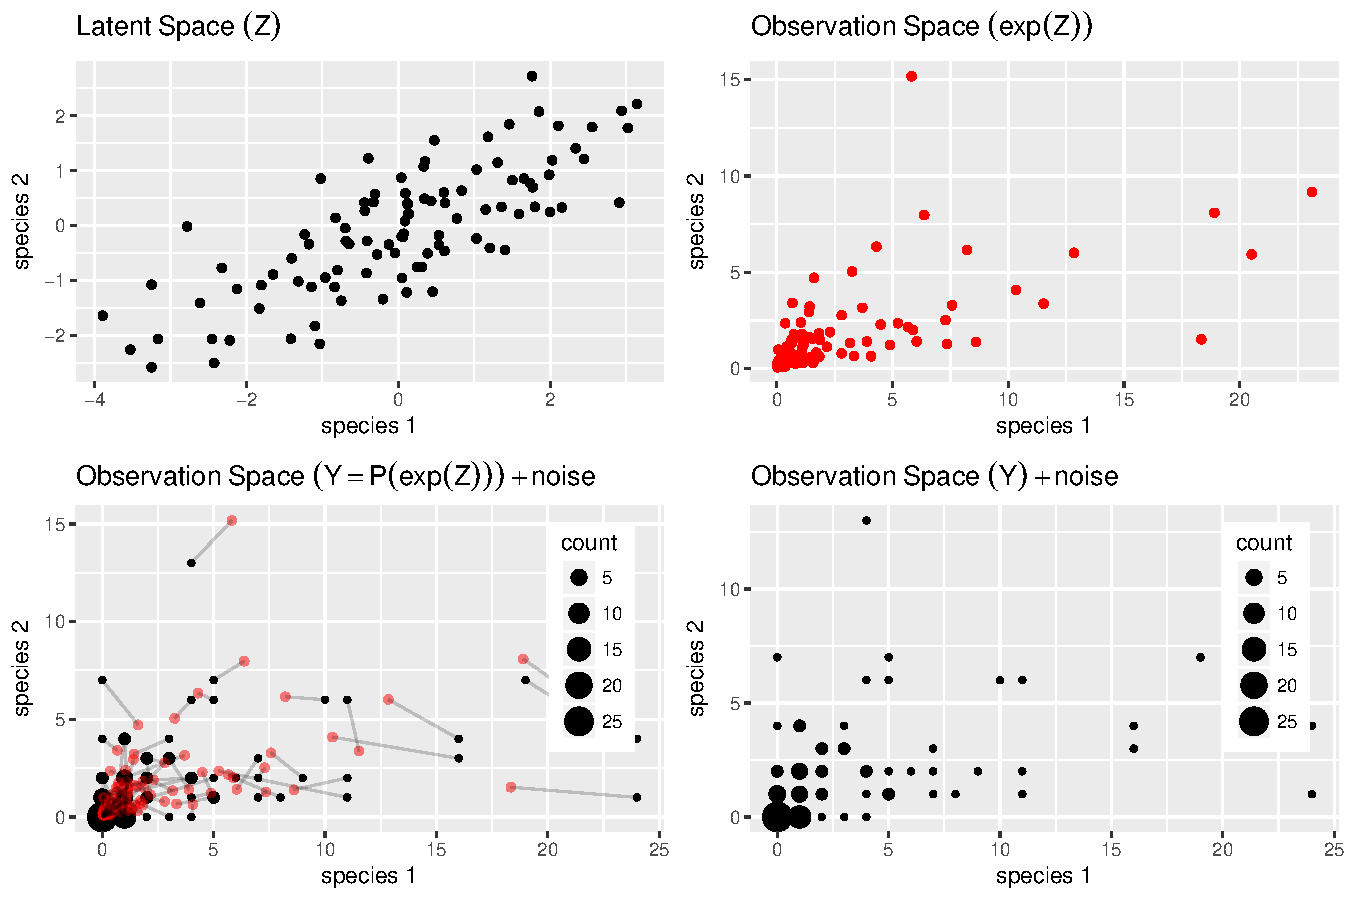
\includegraphics[width=.8\textwidth]{figures/PLN_geom-1} 

\end{knitrout}

\end{frame}

\begin{frame}
  \frametitle{Our contributions}

  \begin{block}{Algorithm/Numerical}
    A variational approach coupled with convex optimization techniques suited to higher dimensional data sets.
    
    \paragraph{{\tt PLNmodels} R/C++-package:}  \text{\url{https://github.com/jchiquet/PLNmodels}}
  \end{block}
  
  \vfill
  
  \begin{block}{Extensions for multivariate analysis}
     \paragraph{Idea:} put some additional constraint on the residual variance.
      \begin{itemize}
      \item \emphase{Network Inference} \\
        \rsa select direct interaction in $\bSigma^{-1}$ via sparsity constraints
        
      \item \textcolor{gray}{\it Principal component analysis}\\
        \textcolor{gray}{\it constraint the rank of $\bSigma$ (most important effect in the variance)}

    \end{itemize}

    \paragraph{Challenge:} a variant of the variational algorithm is required for each model
  \end{block}


\end{frame}



\begin{frame}[fragile]
  \frametitle{PLN-network: unravel important interactions}

  \paragraph{Variable selection of direct effects.}
    \begin{align*}
      \bZ_i \text{ iid} & \sim \clN_p(\bzr_p, \bSigma), & \emphase{\|\bSigma^{-1}\|_1 \leq c} \\
      \bY_i \,|\, \bZ_i & \sim \clP(\exp\{\bO_i + \bX_i \bbeta + \bZ_i\})
      \end{align*}

  \paragraph{Interpretation: conditional independence structure.}
    \begin{equation*}
      (i,j)  \notin  \mathcal{E}  \Leftrightarrow  Z_i  \indep  Z_j  |
      Z_{\backslash \{i,j\}} \Leftrightarrow \bSigma_{ij}^{-1} = 0.
    \end{equation*}

    \begin{center}
      \begin{tabular}{c@{\hspace{2cm}}c}
        \begin{tabular}{c}
          \small $\mathcal{G}=(\mathcal{P},\mathcal{E})$ \\
          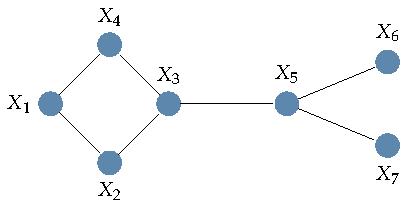
\includegraphics[width=.3\textwidth]{graph}
        \end{tabular}
     &
       \begin{tabular}{c}
         \small $\bSigma^{-1}$\\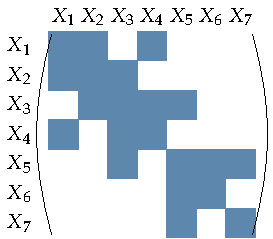
\includegraphics[width=.2\textwidth]{Markovadjacency}
       \end{tabular}
      \end{tabular}
    \end{center}

  \paragraph{PLN-network: find a sparse reconstruction of the latent inverse covariance}
  
    Iterate over variational estimator and Graphical-Lasso [BDE08,YL08,FHT07] in the latent layer

\end{frame}

\begin{frame}[fragile]
  \frametitle{Networks of partial correlations for oak mildew pathobiome}

\begin{knitrout}\scriptsize
\definecolor{shadecolor}{rgb}{0.969, 0.969, 0.969}\color{fgcolor}\begin{kframe}
\begin{alltt}
  \hlcom{# Models with offset and covariates (tree + orientation)}
  \hlstd{formula} \hlkwb{<-} \hlstd{counts} \hlopt{~} \hlnum{1} \hlopt{+} \hlstd{covariates}\hlopt{$}\hlstd{tree} \hlopt{+} \hlstd{covariates}\hlopt{$}\hlstd{orientation} \hlopt{+} \hlkwd{offset}\hlstd{(}\hlkwd{log}\hlstd{(offsets))}
  \hlstd{models_PLN} \hlkwb{<-} \hlkwd{PLNnetwork}\hlstd{(formula,} \hlkwc{penalties} \hlstd{=} \hlnum{10}\hlopt{^}\hlkwd{seq}\hlstd{(}\hlkwd{log10}\hlstd{(}\hlnum{2}\hlstd{),} \hlkwd{log10}\hlstd{(}\hlnum{0.6}\hlstd{),} \hlkwc{len} \hlstd{=} \hlnum{30}\hlstd{))}
\end{alltt}
\end{kframe}
\end{knitrout}


\begin{overprint}
  \foreach\x in{1,...,15}{
    \includegraphics<\x>[trim={2.5cm 2.5cm 2.5cm 2.5cm},clip, width=\textwidth]{figures/plot-networks-\x}
  }
\end{overprint}

\end{frame}

\end{document}
